
\section{Experiments on the Kubernetes Microservices environment}


The \textbf{Kubernetes Microservices} environment is a \emph{real cluster} (1 \textit{worker} node: 8 vCPUs, 32 GB \acn{RAM}, 1 Gbps) used as the input environment for the MAMAD method. A schematic illustration of this cluster and its services is provided in \autoref{fig:k8s_microservices_real}. The cluster hosts an e-commerce web application composed of 4 chained microservices (API, Auth, Products, Orders) orchestrated via Kubernetes. Each service is deployed in a pod with a variable number of replicas (1 to 5). The cluster is {API}, Auth, Products, Orders) orchestrated via Kubernetes. Each service is deployed in a \emph{pod} with a variable number of replicas (1 to 5). The cluster is monitored in real time via Prometheus/Grafana, collecting metrics such as \acn{CPU}/memory usage, request rate, latency, queues, and pod status. Stress test scenarios are applied to simulate real-world conditions: bottlenecks (increased traffic), DDoS attacks (malicious traffic), pod failures (simulated via \textquote{kubectl delete pod}), and resource contention (\acn {CPU}/memory). The goal is to evaluate the agents' ability to maintain the cluster's operational resilience by dynamically adapting resources and responding to incidents. A summary illustration of this type of scenario is provided in \autoref{fig:k8s_cluster_graph_intro}\index{Kubernetes Microservices}.


% ======================================

% \begin{enumerate*}[label={\roman*)}, itemjoin={;\quad}]
\begin{itemize}
\item \textbf{State space:} current state of the actual cluster and the 4 chained services \((i \in \{1..4\})\):
\(
s = \{\text{replicas}^i,\,
U_{\text{cpu}}^i, U_{\text{mem}}^i,\,
T_{\text{in}}^i, T_{\text{out}}^i,\ ,
Q_{\text{pending}}^i,\,
S_{\text{status}}^{i,\text{pods}},\,
P_{\text{priority}}^i\}_{i=1..4}
\)
and global aggregates (average latency \(L_{\text{avg}}\), request rate \(R_{\text{rate}}\), availability)
\item \textbf{Observation space:} partial \emph{actual} observation (\acn{Dec-POMDP}) obtained via the Kubernetes/metrics collection \acn{API}. It is \emph{role-specific}:
\begin{enumerate*}[label={}, itemjoin={;\,}]
  \item bottlenecks: \(Q_{\text{pending}}^i, T_{\text{in}}^i/T_{\text{out}}^i\)
  \item \phantom{XXX} DDoS: \(R_{\text{rate}}, \Delta T, L_{\text{avg}}\)
  \item failures: \(S_{\text{status}}^{i,\text{pods}}, F_{\text{fail}}^i\)
  \ item resources: \(U_{\text{cpu}}^i, U_{\text{mem}}^i, P_{\text{priority}}^i\)
\end{enumerate*}
\item \textbf{Scope of action:} \emph{actual actions} applied to the cluster via the Kubernetes API: \begin{enumerate*}[label={\roman*)}, itemjoin={;\quad}] \item \emph{Targeted scaling}: \textquote{scale\_up}(Kubernetes API): \begin{enumerate*}[label={\roman*)}, itemjoin={;\quad}] \item \emph{Targeted scaling}: \textquote{scale\_up}(Kubernetes {API}~Kubernetes:
\begin{enumerate*}[label={\roman*)}, itemjoin={;\quad}]
  \item \emph{Targeted scaling}: \textquote{scale\_up}(i), \textquote{scale\_down} (i)
  \item \emph{DDoS management}: \textquote{rate\_limit\_ingress}(i), \textquote{isolate\_service}(i)
  \item \emph{Failure recovery}: \textquote{restart\_failed\_pod}(i), \textquote{reschedule\_pod}(i)
  \item \emph{Resource arbitration}: \textquote{throttle\_low\_prio}(i), \textquote{rebalance\_quota}(i)
\end{enumerate*}
\item \textbf{Reward structure:} reward \emph{calculated based on actual telemetry} (QoS/resilience):
\[
  R_{\text{global}}=
  \text{SuccessRate} -w_2\cdot\text{DownTime} -w_3\cdot L_{\text{avg}} -w_4\cdot \text{Resilience} -w_5\cdot \text{Pending} -w_6\cdot \text{Pending\_Time} -w_7\cdot \text{Pending\_Time} -w_8\cdot \text{Pending\_Time} -w_9\cdot \text{Pending\_Time} -w_10\cdot \text{Pending\_Time} -w
  {SuccessRate}
  -w_2\cdot\overline{Q_{\text{pending}}}
  -w_3\cdot L_{\text{avg}}
  -w_4\cdot \text{DownTime}
  -w_5\cdot \text{OverProvision},
\]
supplemented by sub-rewards per role:
\begin{gather*}
  R_{\text{bottleneck}}=-\sum_i Q_{\text{pending}}^i \\
  R_{\text{ddos}}=-(\text{Downtime}\cdot w_d+L_{\text{avg}}\cdot w_l) \\
  R_{\text{failure}}=-\sum_i T_{\text{downtime}}^i \\
  R_{\text{resource}}=-\sum_{i\in\text{Critical}}(U_{\text{cpu}}^i+U_{\text{mem}}^i)
\end{gather*}

\item \textbf{Objective:} maximize the \emph{operational resilience} of the actual cluster (high success rate, low latency/queues, maximum availability) under 5 scenarios: bottlenecks, DDoS, pod failures, resource contention, \emph{mixed}
% \end{enumerate*}
\end {itemize}

% ======================================

\noindent\textbf{Organizational specifications:}
% \begin{enumerate*}[label={\roman*)}, itemjoin={;\quad}]
\begin {itemize}
\item \textbf{Roles:} \textquote{Bottleneck Manager}, \textquote{DDoS Manager}, \textquote{Outage Manager}, \textquote{Resource Manager}
\item \textbf{Tasks:}
\(\langle\)minimize \(Q_{\text{pending}}^i\)\(\rangle\);
\(\langle\)detect/isolate DDoS and reduce downtime/latency\(\rangle\);
\(\langle\)\(\downarrow T_{\text{downtime}}\) through rapid recovery\(\rangle\);
\(\langle\)prioritize critical services under \(U_{\text{cpu/mem}}\) constraint\(\rangle\)
\item \textbf{Constraints:}
(a) \emph{deontic} by role (e.g., only \textquote{DDoS Manager} can \textquote{isolate\_ \allowbreak service});
(b) \emph{segregation of responsibilities} (avoid contradictory \textquote{scale\_up});
(c) \emph{QoS safeguards} (\(Q_{\text{pending}}^i<Q_{\text{threshold}}, U_{\text{cpu}}^{\text{total}}<U_{\text{threshold}}\));
(d) two integration modes during training: \textit{hard constraints} (action masking) vs. \textit{soft constraints} (reward shaping)
% \end{enumerate*}
\end{itemize}

\medskip
\noindent\textit{Note (specificity \textquote{real}):}
% \begin{enumerate*}[label={--}, itemjoin={\quad}]
\begin{itemize}
  \item \textsc{MOD/TRN} on digital twin derived from real cluster traces;
  \item \textsc{TRF}: deployment of policies learned on the cluster via the Kubernetes API; {API};
  \item operational security: bounded actions (quotas/limits), rollbacks, and rate limiting to preserve QoS.
        % \end{enumerate*}
\end{itemize}

\begin{figure}[h!]
  \centering
  \includegraphics[trim=1.8cm 3.3cm 1.25cm 3.5cm, clip, width=\linewidth]{figures/k8s_cluster_graph.pdf}
  \caption{Real cluster \textquote{Chained services} (4 services) and levers of action exposed to CybMASDE/MAMAD via the Kubernetes API.}
  \label{fig:k8s_microservices_real}
\end{figure}

\begin{figure}[h!]
  \centering
  \hspace{-0.4cm}
  \includegraphics[trim=0cm 0cm 0cm 0cm, clip, width=\textwidth]{figures/scenario_introduction.pdf}
  \caption [An abstract view of the Kubernetes cluster scenario]{An abstract view of the Kubernetes cluster scenario where each service runs in pods managed by \textit{Deployments} and can be dynamically replicated. Defender agents with specific roles (e.g., \textit{DDoS detector}, \textit{resource manager}, \textit{bottleneck manager}, \textit{failure manager}) continuously monitor key metrics (latency, pending requests, incoming/outgoing traffic, pod states, \acn{CPU}/memory usage) and apply via the \ acn{API} to adjust replicas, isolate affected services, or restart failed components. The illustration highlights four types of disruptions targeting the chain (\textit{bottleneck}, \textit{contention} (resource conflict), \textit{crash} (pod failure), and \textit{DDoS}/massive injections), as well as pod compromises. Agents must detect anomalies, isolate/segment compromised components, and reallocate resources to preserve overall operational resilience (availability, throughput, latency) and minimize the impact on end users.
  \label{fig:k8s_cluster_graph_intro}
\end{figure}


\subsection{Description of the experimental protocol instance}

\paragraph{1. Initial configuration}

We operate \emph{on the actual cluster} (no command line simulation playing the role of the \textquote{actual environment}). The cluster (\textbf{\acn{VM} 8~vCPU, 32 GB \acn{RAM}, 1 Gbps}) hosts the e-commerce application (4 microservices in a chain). Telemetry is collected by \textit{Prometheus} and visualized via \textit{Grafana}. \textquote{CybMASDE}/\textquote{KARMA} interfaces with the Kubernetes \acn{API} to \textit {observe} the status and \textit{act} (scaling, isolation, restart). A \textbf{digital twin} is built from the traces to train the policies offline, which are then \textbf{transferred} and \textit{closed in a loop} on the cluster (iterative learning by refreshing traces).

\begin{figure}[h!]
  \centering
  \resizebox{\textwidth}{!}{%
    


\tikzset{every picture/.style={line width=0.75pt}} %set default line width to 0.75pt        

\begin{tikzpicture}[x=0.75pt,y=0.75pt,yscale=-1.2,xscale=1.2]
%uncomment if require: \path (0,1414); %set diagram left start at 0, and has height of 1414

%Straight Lines [id:da5609883377896374] 
\draw [color={rgb, 255:red, 74; green, 144; blue, 226 }  ,draw opacity=1 ][line width=2.25]    (317.22,111.13) -- (360.07,111.13) ;
\draw [shift={(365.07,111.13)}, rotate = 180] [fill={rgb, 255:red, 74; green, 144; blue, 226 }  ,fill opacity=1 ][line width=0.08]  [draw opacity=0] (5.72,-2.75) -- (0,0) -- (5.72,2.75) -- cycle    ;
%Image [id:dp9396292457736715] 
\draw (106.77,60.95) node  {\includegraphics[width=18.66pt,height=18.36pt]{figures/karma_architecture/pod.png}};
%Image [id:dp3874378335758297] 
\draw (145.86,60.95) node  {\includegraphics[width=18.66pt,height=18.36pt]{figures/karma_architecture/pod.png}};
%Shape: Rectangle [id:dp4562827234223257] 
\draw  [color={rgb, 255:red, 74; green, 144; blue, 226 }  ,draw opacity=1 ][line width=1.5]  (89,28.36) .. controls (89,25.6) and (91.24,23.36) .. (94,23.36) -- (255,23.36) .. controls (257.76,23.36) and (260,25.6) .. (260,28.36) -- (260,132) .. controls (260,134.76) and (257.76,137) .. (255,137) -- (94,137) .. controls (91.24,137) and (89,134.76) .. (89,132) -- cycle ;
%Image [id:dp9455935833751838] 
\draw (172.5,16.24) node  {\includegraphics[width=18.66pt,height=18.36pt]{figures/karma_architecture/kubernetes.png}};
%Shape: Rectangle [id:dp9564725691593288] 
\draw  [color={rgb, 255:red, 74; green, 144; blue, 226 }  ,draw opacity=1 ][line width=1.5]  (92.55,50.21) .. controls (92.55,47.45) and (94.79,45.21) .. (97.55,45.21) -- (155.08,45.21) .. controls (157.84,45.21) and (160.08,47.45) .. (160.08,50.21) -- (160.08,70.81) .. controls (160.08,73.57) and (157.84,75.81) .. (155.08,75.81) -- (97.55,75.81) .. controls (94.79,75.81) and (92.55,73.57) .. (92.55,70.81) -- cycle ;
%Image [id:dp9120856447688912] 
\draw (126.32,39.97) node  {\includegraphics[width=18.66pt,height=18.36pt]{figures/karma_architecture/node.png}};
%Image [id:dp5738167237736518] 
\draw (106.77,119.52) node  {\includegraphics[width=18.66pt,height=18.36pt]{figures/karma_architecture/pod.png}};
%Image [id:dp2199681121060142] 
\draw (145.86,119.52) node  {\includegraphics[width=18.66pt,height=18.36pt]{figures/karma_architecture/pod.png}};
%Shape: Rectangle [id:dp12159705904547402] 
\draw  [color={rgb, 255:red, 74; green, 144; blue, 226 }  ,draw opacity=1 ][line width=1.5]  (92.55,108.78) .. controls (92.55,106.02) and (94.79,103.78) .. (97.55,103.78) -- (155.08,103.78) .. controls (157.84,103.78) and (160.08,106.02) .. (160.08,108.78) -- (160.08,129.38) .. controls (160.08,132.14) and (157.84,134.38) .. (155.08,134.38) -- (97.55,134.38) .. controls (94.79,134.38) and (92.55,132.14) .. (92.55,129.38) -- cycle ;
%Image [id:dp37768653229718074] 
\draw (126.32,98.54) node  {\includegraphics[width=18.66pt,height=18.36pt]{figures/karma_architecture/node.png}};
%Shape: Rectangle [id:dp20840815212238661] 
\draw  [color={rgb, 255:red, 74; green, 144; blue, 226 }  ,draw opacity=1 ][line width=1.5]  (264,28.36) .. controls (264,25.6) and (266.24,23.36) .. (269,23.36) -- (411.78,23.36) .. controls (414.54,23.36) and (416.78,25.6) .. (416.78,28.36) -- (416.78,132) .. controls (416.78,134.76) and (414.54,137) .. (411.78,137) -- (269,137) .. controls (266.24,137) and (264,134.76) .. (264,132) -- cycle ;
%Straight Lines [id:da9232180983272227] 
\draw [color={rgb, 255:red, 74; green, 144; blue, 226 }  ,draw opacity=1 ][line width=2.25]    (164,112) -- (201,112) ;
\draw [shift={(206,112)}, rotate = 180] [fill={rgb, 255:red, 74; green, 144; blue, 226 }  ,fill opacity=1 ][line width=0.08]  [draw opacity=0] (5.72,-2.75) -- (0,0) -- (5.72,2.75) -- cycle    ;
%Straight Lines [id:da6082715106712999] 
\draw [color={rgb, 255:red, 74; green, 144; blue, 226 }  ,draw opacity=1 ][line width=2.25]    (180,90.22) -- (167,90.22) ;
\draw [shift={(162,90.22)}, rotate = 360] [fill={rgb, 255:red, 74; green, 144; blue, 226 }  ,fill opacity=1 ][line width=0.08]  [draw opacity=0] (5.72,-2.75) -- (0,0) -- (5.72,2.75) -- cycle    ;
%Straight Lines [id:da30764510910060716] 
\draw [color={rgb, 255:red, 74; green, 144; blue, 226 }  ,draw opacity=1 ][line width=2.25]    (210,72) -- (199,72) ;
\draw [shift={(194,72)}, rotate = 360] [fill={rgb, 255:red, 74; green, 144; blue, 226 }  ,fill opacity=1 ][line width=0.08]  [draw opacity=0] (5.72,-2.75) -- (0,0) -- (5.72,2.75) -- cycle    ;
%Straight Lines [id:da5394403186779959] 
\draw [color={rgb, 255:red, 74; green, 144; blue, 226 }  ,draw opacity=1 ][line width=2.25]    (178,56.22) -- (167,56.22) ;
\draw [shift={(162,56.22)}, rotate = 360] [fill={rgb, 255:red, 74; green, 144; blue, 226 }  ,fill opacity=1 ][line width=0.08]  [draw opacity=0] (5.72,-2.75) -- (0,0) -- (5.72,2.75) -- cycle    ;
%Straight Lines [id:da6399475815904785] 
\draw [color={rgb, 255:red, 74; green, 144; blue, 226 }  ,draw opacity=1 ][line width=2.25]    (272,72) -- (235,72) ;
\draw [shift={(230,72)}, rotate = 360] [fill={rgb, 255:red, 74; green, 144; blue, 226 }  ,fill opacity=1 ][line width=0.08]  [draw opacity=0] (5.72,-2.75) -- (0,0) -- (5.72,2.75) -- cycle    ;
%Straight Lines [id:da24320102833940327] 
\draw [color={rgb, 255:red, 74; green, 144; blue, 226 }  ,draw opacity=1 ][line width=2.25]    (267,112) -- (230,112) ;
\draw [shift={(272,112)}, rotate = 180] [fill={rgb, 255:red, 74; green, 144; blue, 226 }  ,fill opacity=1 ][line width=0.08]  [draw opacity=0] (5.72,-2.75) -- (0,0) -- (5.72,2.75) -- cycle    ;
%Shape: Rectangle [id:dp9149123987409296] 
\draw  [color={rgb, 255:red, 255; green, 255; blue, 255 }  ,draw opacity=1 ][fill={rgb, 255:red, 255; green, 255; blue, 255 }  ,fill opacity=1 ] (328.83,106.67) -- (353.11,106.67) -- (353.11,114) -- (328.83,114) -- cycle ;
%Image [id:dp7127891043436136] 
\draw (341.68,109.47) node  {\includegraphics[width=14.57pt,height=15.21pt]{figures/karma_architecture/pettingzoo.png}};
%Straight Lines [id:da5757027637146572] 
\draw [color={rgb, 255:red, 74; green, 144; blue, 226 }  ,draw opacity=1 ][line width=2.25]    (357.9,41) -- (364.9,41) ;
\draw [shift={(352.9,41)}, rotate = 0] [fill={rgb, 255:red, 74; green, 144; blue, 226 }  ,fill opacity=1 ][line width=0.08]  [draw opacity=0] (5.72,-2.75) -- (0,0) -- (5.72,2.75) -- cycle    ;
%Straight Lines [id:da29364722138505184] 
\draw [color={rgb, 255:red, 74; green, 144; blue, 226 }  ,draw opacity=1 ][line width=2.25]    (390.99,97.77) -- (390.99,57.25) ;
\draw [shift={(390.99,52.25)}, rotate = 90] [fill={rgb, 255:red, 74; green, 144; blue, 226 }  ,fill opacity=1 ][line width=0.08]  [draw opacity=0] (5.72,-2.75) -- (0,0) -- (5.72,2.75) -- cycle    ;
%Straight Lines [id:da5470457469462804] 
\draw [color={rgb, 255:red, 74; green, 144; blue, 226 }  ,draw opacity=1 ][line width=2.25]    (390.9,71) -- (325.9,71) ;
\draw [shift={(320.9,71)}, rotate = 360] [fill={rgb, 255:red, 74; green, 144; blue, 226 }  ,fill opacity=1 ][line width=0.08]  [draw opacity=0] (5.72,-2.75) -- (0,0) -- (5.72,2.75) -- cycle    ;
%Shape: Rectangle [id:dp8476965567779329] 
\draw  [color={rgb, 255:red, 255; green, 255; blue, 255 }  ,draw opacity=1 ][fill={rgb, 255:red, 255; green, 255; blue, 255 }  ,fill opacity=1 ] (378.41,65.11) -- (397.83,65.11) -- (397.83,92) -- (378.41,92) -- cycle ;
%Shape: Smiley Face [id:dp8656850497140396] 
\draw  [fill={rgb, 255:red, 255; green, 255; blue, 255 }  ,fill opacity=1 ][line width=0.75]  (380.35,69.4) .. controls (380.35,67.3) and (382.09,65.6) .. (384.24,65.6) .. controls (386.38,65.6) and (388.12,67.3) .. (388.12,69.4) .. controls (388.12,71.5) and (386.38,73.2) .. (384.24,73.2) .. controls (382.09,73.2) and (380.35,71.5) .. (380.35,69.4) -- cycle ; \draw  [fill={rgb, 255:red, 255; green, 255; blue, 255 }  ,fill opacity=1 ][line width=0.75]  (382.53,68.11) .. controls (382.53,67.9) and (382.7,67.73) .. (382.92,67.73) .. controls (383.13,67.73) and (383.31,67.9) .. (383.31,68.11) .. controls (383.31,68.32) and (383.13,68.49) .. (382.92,68.49) .. controls (382.7,68.49) and (382.53,68.32) .. (382.53,68.11) -- cycle ; \draw  [fill={rgb, 255:red, 255; green, 255; blue, 255 }  ,fill opacity=1 ][line width=0.75]  (385.17,68.11) .. controls (385.17,67.9) and (385.34,67.73) .. (385.56,67.73) .. controls (385.77,67.73) and (385.95,67.9) .. (385.95,68.11) .. controls (385.95,68.32) and (385.77,68.49) .. (385.56,68.49) .. controls (385.34,68.49) and (385.17,68.32) .. (385.17,68.11) -- cycle ; \draw  [line width=0.75]  (382.29,70.92) .. controls (383.59,71.94) and (384.88,71.94) .. (386.18,70.92) ;
%Shape: Smiley Face [id:dp9163740789669144] 
\draw  [fill={rgb, 255:red, 255; green, 255; blue, 255 }  ,fill opacity=1 ][line width=0.75]  (392.01,69.4) .. controls (392.01,67.3) and (393.75,65.6) .. (395.89,65.6) .. controls (398.04,65.6) and (399.78,67.3) .. (399.78,69.4) .. controls (399.78,71.5) and (398.04,73.2) .. (395.89,73.2) .. controls (393.75,73.2) and (392.01,71.5) .. (392.01,69.4) -- cycle ; \draw  [fill={rgb, 255:red, 255; green, 255; blue, 255 }  ,fill opacity=1 ][line width=0.75]  (394.18,68.11) .. controls (394.18,67.9) and (394.36,67.73) .. (394.57,67.73) .. controls (394.79,67.73) and (394.96,67.9) .. (394.96,68.11) .. controls (394.96,68.32) and (394.79,68.49) .. (394.57,68.49) .. controls (394.36,68.49) and (394.18,68.32) .. (394.18,68.11) -- cycle ; \draw  [fill={rgb, 255:red, 255; green, 255; blue, 255 }  ,fill opacity=1 ][line width=0.75]  (396.82,68.11) .. controls (396.82,67.9) and (397,67.73) .. (397.21,67.73) .. controls (397.43,67.73) and (397.6,67.9) .. (397.6,68.11) .. controls (397.6,68.32) and (397.43,68.49) .. (397.21,68.49) .. controls (397,68.49) and (396.82,68.32) .. (396.82,68.11) -- cycle ; \draw  [line width=0.75]  (393.95,70.92) .. controls (395.24,71.94) and (396.54,71.94) .. (397.83,70.92) ;
%Shape: Smiley Face [id:dp8186451078369623] 
\draw  [fill={rgb, 255:red, 255; green, 255; blue, 255 }  ,fill opacity=1 ][line width=0.75]  (386.18,77.44) .. controls (386.18,75.34) and (387.92,73.64) .. (390.06,73.64) .. controls (392.21,73.64) and (393.95,75.34) .. (393.95,77.44) .. controls (393.95,79.54) and (392.21,81.24) .. (390.06,81.24) .. controls (387.92,81.24) and (386.18,79.54) .. (386.18,77.44) -- cycle ; \draw  [fill={rgb, 255:red, 255; green, 255; blue, 255 }  ,fill opacity=1 ][line width=0.75]  (388.36,76.15) .. controls (388.36,75.94) and (388.53,75.77) .. (388.74,75.77) .. controls (388.96,75.77) and (389.13,75.94) .. (389.13,76.15) .. controls (389.13,76.36) and (388.96,76.53) .. (388.74,76.53) .. controls (388.53,76.53) and (388.36,76.36) .. (388.36,76.15) -- cycle ; \draw  [fill={rgb, 255:red, 255; green, 255; blue, 255 }  ,fill opacity=1 ][line width=0.75]  (391,76.15) .. controls (391,75.94) and (391.17,75.77) .. (391.39,75.77) .. controls (391.6,75.77) and (391.77,75.94) .. (391.77,76.15) .. controls (391.77,76.36) and (391.6,76.53) .. (391.39,76.53) .. controls (391.17,76.53) and (391,76.36) .. (391,76.15) -- cycle ; \draw  [line width=0.75]  (388.12,78.96) .. controls (389.42,79.98) and (390.71,79.98) .. (392.01,78.96) ;
%Flowchart: Punched Tape [id:dp6020643269389074] 
\draw  [fill={rgb, 255:red, 255; green, 255; blue, 255 }  ,fill opacity=1 ] (313.9,33.81) .. controls (313.9,35.03) and (318.18,36.02) .. (323.45,36.02) .. controls (328.73,36.02) and (333,35.03) .. (333,33.81) .. controls (333,32.58) and (337.28,31.59) .. (342.55,31.59) .. controls (347.83,31.59) and (352.1,32.58) .. (352.1,33.81) -- (352.1,51.52) .. controls (352.1,50.3) and (347.83,49.31) .. (342.55,49.31) .. controls (337.28,49.31) and (333,50.3) .. (333,51.52) .. controls (333,52.75) and (328.73,53.74) .. (323.45,53.74) .. controls (318.18,53.74) and (313.9,52.75) .. (313.9,51.52) -- cycle ;
%Straight Lines [id:da950307097731951] 
\draw [line width=0.75]    (324.14,41.04) -- (341.9,41) ;
%Shape: Smiley Face [id:dp8914579811118104] 
\draw  [line width=0.75]  (320.58,40.88) .. controls (320.58,39.7) and (321.59,38.73) .. (322.85,38.73) .. controls (324.1,38.73) and (325.11,39.7) .. (325.11,40.88) .. controls (325.11,42.07) and (324.1,43.03) .. (322.85,43.03) .. controls (321.59,43.03) and (320.58,42.07) .. (320.58,40.88) -- cycle ; \draw  [line width=0.75]  (321.85,40.15) .. controls (321.85,40.03) and (321.95,39.94) .. (322.08,39.94) .. controls (322.2,39.94) and (322.3,40.03) .. (322.3,40.15) .. controls (322.3,40.27) and (322.2,40.37) .. (322.08,40.37) .. controls (321.95,40.37) and (321.85,40.27) .. (321.85,40.15) -- cycle ; \draw  [line width=0.75]  (323.39,40.15) .. controls (323.39,40.03) and (323.49,39.94) .. (323.62,39.94) .. controls (323.74,39.94) and (323.84,40.03) .. (323.84,40.15) .. controls (323.84,40.27) and (323.74,40.37) .. (323.62,40.37) .. controls (323.49,40.37) and (323.39,40.27) .. (323.39,40.15) -- cycle ; \draw  [line width=0.75]  (321.71,41.74) .. controls (322.47,42.31) and (323.22,42.31) .. (323.98,41.74) ;
%Shape: Smiley Face [id:dp07941198495535606] 
\draw  [line width=0.75]  (329.9,45.15) .. controls (329.9,43.96) and (330.92,43) .. (332.17,43) .. controls (333.42,43) and (334.44,43.96) .. (334.44,45.15) .. controls (334.44,46.33) and (333.42,47.29) .. (332.17,47.29) .. controls (330.92,47.29) and (329.9,46.33) .. (329.9,45.15) -- cycle ; \draw  [line width=0.75]  (331.17,44.42) .. controls (331.17,44.3) and (331.28,44.2) .. (331.4,44.2) .. controls (331.53,44.2) and (331.63,44.3) .. (331.63,44.42) .. controls (331.63,44.54) and (331.53,44.63) .. (331.4,44.63) .. controls (331.28,44.63) and (331.17,44.54) .. (331.17,44.42) -- cycle ; \draw  [line width=0.75]  (332.72,44.42) .. controls (332.72,44.3) and (332.82,44.2) .. (332.94,44.2) .. controls (333.07,44.2) and (333.17,44.3) .. (333.17,44.42) .. controls (333.17,44.54) and (333.07,44.63) .. (332.94,44.63) .. controls (332.82,44.63) and (332.72,44.54) .. (332.72,44.42) -- cycle ; \draw  [line width=0.75]  (331.04,46.01) .. controls (331.79,46.58) and (332.55,46.58) .. (333.3,46.01) ;
%Shape: Smiley Face [id:dp8353415903298282] 
\draw  [line width=0.75]  (341.9,40.85) .. controls (341.9,39.67) and (342.92,38.71) .. (344.17,38.71) .. controls (345.42,38.71) and (346.44,39.67) .. (346.44,40.85) .. controls (346.44,42.04) and (345.42,43) .. (344.17,43) .. controls (342.92,43) and (341.9,42.04) .. (341.9,40.85) -- cycle ; \draw  [line width=0.75]  (343.17,40.12) .. controls (343.17,40) and (343.28,39.91) .. (343.4,39.91) .. controls (343.53,39.91) and (343.63,40) .. (343.63,40.12) .. controls (343.63,40.24) and (343.53,40.34) .. (343.4,40.34) .. controls (343.28,40.34) and (343.17,40.24) .. (343.17,40.12) -- cycle ; \draw  [line width=0.75]  (344.72,40.12) .. controls (344.72,40) and (344.82,39.91) .. (344.94,39.91) .. controls (345.07,39.91) and (345.17,40) .. (345.17,40.12) .. controls (345.17,40.24) and (345.07,40.34) .. (344.94,40.34) .. controls (344.82,40.34) and (344.72,40.24) .. (344.72,40.12) -- cycle ; \draw  [line width=0.75]  (343.04,41.71) .. controls (343.79,42.28) and (344.55,42.28) .. (345.3,41.71) ;
%Straight Lines [id:da21936285199788075] 
\draw [line width=0.75]    (324.19,41.87) -- (329.9,45) ;
%Image [id:dp05694376090002984] 
\draw (218.44,70.24) node  {\includegraphics[width=18.66pt,height=18.36pt]{figures/karma_architecture/api.png}};
%Image [id:dp7747210194064744] 
\draw (186.74,54.54) node  {\includegraphics[width=18.66pt,height=18.36pt]{figures/karma_architecture/deploy.png}};
%Image [id:dp5268588430037433] 
\draw (186.74,87.76) node  {\includegraphics[width=18.66pt,height=18.36pt]{figures/karma_architecture/deploy.png}};
%Image [id:dp7447308292951857] 
\draw (218.44,111.76) node  {\includegraphics[width=18.66pt,height=18.36pt]{figures/karma_architecture/prometheus.png}};
%Shape: Rectangle [id:dp7837974954754439] 
\draw  [color={rgb, 255:red, 75; green, 101; blue, 225 }  ,draw opacity=1 ][fill={rgb, 255:red, 74; green, 144; blue, 226 }  ,fill opacity=1 ] (202.37,94.64) -- (208.29,94.64) -- (208.29,101.67) -- (202.37,101.67) -- cycle ;
%Shape: Rectangle [id:dp780870970882084] 
\draw  [color={rgb, 255:red, 75; green, 101; blue, 225 }  ,draw opacity=1 ][fill={rgb, 255:red, 74; green, 144; blue, 226 }  ,fill opacity=1 ] (286.37,126) -- (292.29,126) -- (292.29,133.03) -- (286.37,133.03) -- cycle ;

%Shape: Rectangle [id:dp7051683429553395] 
\draw  [color={rgb, 255:red, 75; green, 101; blue, 225 }  ,draw opacity=1 ][fill={rgb, 255:red, 74; green, 144; blue, 226 }  ,fill opacity=1 ] (397.37,124.64) -- (403.29,124.64) -- (403.29,131.67) -- (397.37,131.67) -- cycle ;

%Shape: Rectangle [id:dp5578959475333973] 
\draw  [color={rgb, 255:red, 75; green, 101; blue, 225 }  ,draw opacity=1 ][fill={rgb, 255:red, 74; green, 144; blue, 226 }  ,fill opacity=1 ] (368.37,54.64) -- (374.29,54.64) -- (374.29,61.67) -- (368.37,61.67) -- cycle ;

%Shape: Rectangle [id:dp2822949836407178] 
\draw  [color={rgb, 255:red, 75; green, 101; blue, 225 }  ,draw opacity=1 ][fill={rgb, 255:red, 74; green, 144; blue, 226 }  ,fill opacity=1 ] (324.37,78) -- (330.29,78) -- (330.29,85.03) -- (324.37,85.03) -- cycle ;

%Shape: Rectangle [id:dp9339299822588341] 
\draw  [color={rgb, 255:red, 75; green, 101; blue, 225 }  ,draw opacity=1 ][fill={rgb, 255:red, 74; green, 144; blue, 226 }  ,fill opacity=1 ] (205.37,48) -- (211.29,48) -- (211.29,55.03) -- (205.37,55.03) -- cycle ;



% Text Node
\draw (205.5,98.5) node  [font=\fontsize{0.33em}{0.4em}\selectfont,color={rgb, 255:red, 255; green, 255; blue, 255 }  ,opacity=1 ] [align=left] {1};
% Text Node
\draw (244,58.5) node  [font=\normalsize] [align=left] {{\tiny Scaling}};
\draw (244,64.5) node  [font=\normalsize] [align=left] {{\tiny actions}};
% Text Node
\draw (244,99.5) node  [font=\normalsize] [align=left] {{\tiny Metrics}};
\draw (244,105.5) node  [font=\normalsize] [align=left] {{\tiny data}};
% Text Node
\draw (344.5,36) node  [font=\fontsize{0.33em}{0.4em}\selectfont] [align=left] {\begin{minipage}[lt]{8.66pt}\setlength\topsep{0pt}
\begin{center}
{\fontsize{0.33em}{0.4em}\selectfont $\displaystyle \mathbf{\textcolor[rgb]{0.82,0.01,0.11}{\pi }\textcolor[rgb]{0.82,0.01,0.11}{_{3}}}$}
\end{center}

\end{minipage}};
% Text Node
\draw (341,46.5) node  [font=\fontsize{0.33em}{0.4em}\selectfont] [align=left] {\begin{minipage}[lt]{8.66pt}\setlength\topsep{0pt}
\begin{center}
{\fontsize{0.33em}{0.4em}\selectfont $\displaystyle \mathbf{\textcolor[rgb]{0.82,0.01,0.11}{\pi }\textcolor[rgb]{0.82,0.01,0.11}{_{2}}}$}
\end{center}

\end{minipage}};
% Text Node
\draw (320.9,48) node  [font=\fontsize{0.33em}{0.4em}\selectfont] [align=left] {\begin{minipage}[lt]{8.66pt}\setlength\topsep{0pt}
\begin{center}
{\fontsize{0.33em}{0.4em}\selectfont $\displaystyle \mathbf{\textcolor[rgb]{0.82,0.01,0.11}{\pi }\textcolor[rgb]{0.82,0.01,0.11}{_{1}}}$}
\end{center}

\end{minipage}};
% Text Node
\draw  [color={rgb, 255:red, 75; green, 101; blue, 225 }  ,draw opacity=1 ][fill={rgb, 255:red, 136; green, 197; blue, 246 }  ,fill opacity=1 ][line width=1.5]   (322.77,14.89) .. controls (322.77,13.78) and (323.67,12.89) .. (324.77,12.89) -- (355.77,12.89) .. controls (356.88,12.89) and (357.77,13.78) .. (357.77,14.89) -- (357.77,26.89) .. controls (357.77,27.99) and (356.88,28.89) .. (355.77,28.89) -- (324.77,28.89) .. controls (323.67,28.89) and (322.77,27.99) .. (322.77,26.89) -- cycle  ;
\draw (340.27,20.89) node  [font=\tiny] [align=left] {\begin{minipage}[lt]{21.5pt}\setlength\topsep{0pt}
\begin{center}
KARMA
\end{center}

\end{minipage}};
% Text Node
\draw (290,40.5) node  [font=\tiny] [align=left] {\begin{minipage}[lt]{27.24pt}\setlength\topsep{0pt}
\begin{center}
Organizational\\Analysis
\end{center}

\end{minipage}};
% Text Node
\draw (388,86.39) node  [font=\tiny] [align=left] {\begin{minipage}[lt]{43.42pt}\setlength\topsep{0pt}
\begin{center}
Trained policies
\end{center}

\end{minipage}};
% Text Node
\draw (344.13,127.35) node  [font=\tiny] [align=left] {\begin{minipage}[lt]{60.78pt}\setlength\topsep{0pt}
\begin{center}
PettingZoo environment
\end{center}

\end{minipage}};
% Text Node
\draw (218,127) node  [font=\tiny] [align=left] {\begin{minipage}[lt]{30.31pt}\setlength\topsep{0pt}
\begin{center}
Prometheus
\end{center}

\end{minipage}};
% Text Node
\draw  [color={rgb, 255:red, 75; green, 101; blue, 225 }  ,draw opacity=1 ][fill={rgb, 255:red, 136; green, 197; blue, 246 }  ,fill opacity=1 ][line width=1.5]   (272.9,62) .. controls (272.9,60.9) and (273.8,60) .. (274.9,60) -- (317.9,60) .. controls (319.01,60) and (319.9,60.9) .. (319.9,62) -- (319.9,83) .. controls (319.9,84.1) and (319.01,85) .. (317.9,85) -- (274.9,85) .. controls (273.8,85) and (272.9,84.1) .. (272.9,83) -- cycle  ;
\draw (296.4,72.5) node  [font=\tiny,color={rgb, 255:red, 0; green, 0; blue, 0 }  ,opacity=1 ] [align=left] {Transfer\\Component};
% Text Node
\draw  [color={rgb, 255:red, 75; green, 101; blue, 225 }  ,draw opacity=1 ][fill={rgb, 255:red, 136; green, 197; blue, 246 }  ,fill opacity=1 ][line width=1.5]   (365.88,29.46) .. controls (365.88,28.35) and (366.78,27.46) .. (367.88,27.46) -- (410.88,27.46) .. controls (411.99,27.46) and (412.88,28.35) .. (412.88,29.46) -- (412.88,50.46) .. controls (412.88,51.56) and (411.99,52.46) .. (410.88,52.46) -- (367.88,52.46) .. controls (366.78,52.46) and (365.88,51.56) .. (365.88,50.46) -- cycle  ;
\draw (389.38,39.96) node  [font=\tiny,color={rgb, 255:red, 0; green, 0; blue, 0 }  ,opacity=1 ] [align=left] {Analyzing\\Component};
% Text Node
\draw  [color={rgb, 255:red, 75; green, 101; blue, 225 }  ,draw opacity=1 ][fill={rgb, 255:red, 136; green, 197; blue, 246 }  ,fill opacity=1 ][line width=1.5]   (365.88,98.24) .. controls (365.88,97.13) and (366.78,96.24) .. (367.88,96.24) -- (410.88,96.24) .. controls (411.99,96.24) and (412.88,97.13) .. (412.88,98.24) -- (412.88,119.24) .. controls (412.88,120.34) and (411.99,121.24) .. (410.88,121.24) -- (367.88,121.24) .. controls (366.78,121.24) and (365.88,120.34) .. (365.88,119.24) -- cycle  ;
\draw (389.38,108.74) node  [font=\tiny,color={rgb, 255:red, 0; green, 0; blue, 0 }  ,opacity=1 ] [align=left] {Training\\Component};
% Text Node
\draw (172.5,33.36) node  [font=\tiny] [align=left] {\begin{minipage}[lt]{16.92pt}\setlength\topsep{0pt}
\begin{center}
Cluster
\end{center}

\end{minipage}};
% Text Node
\draw  [color={rgb, 255:red, 75; green, 101; blue, 225 }  ,draw opacity=1 ][fill={rgb, 255:red, 136; green, 197; blue, 246 }  ,fill opacity=1 ][line width=1.5]   (272.9,99) .. controls (272.9,97.9) and (273.8,97) .. (274.9,97) -- (317.9,97) .. controls (319.01,97) and (319.9,97.9) .. (319.9,99) -- (319.9,120) .. controls (319.9,121.1) and (319.01,122) .. (317.9,122) -- (274.9,122) .. controls (273.8,122) and (272.9,121.1) .. (272.9,120) -- cycle  ;
\draw (296.4,109.5) node  [font=\tiny,color={rgb, 255:red, 0; green, 0; blue, 0 }  ,opacity=1 ] [align=left] {Modeling\\Component};
% Text Node
\draw (173,73.72) node  [font=\tiny,rotate=-90] [align=left] {{\LARGE {\fontfamily{helvet}\selectfont \textcolor[rgb]{0.29,0.56,0.89}{...}}}};
% Text Node
\draw (125.61,118.47) node  [font=\tiny] [align=left] {{\LARGE {\fontfamily{helvet}\selectfont \textcolor[rgb]{0.29,0.56,0.89}{...}}}};
% Text Node
\draw (147,89.5) node  [font=\tiny,rotate=-90] [align=left] {{\LARGE {\fontfamily{helvet}\selectfont \textcolor[rgb]{0.29,0.56,0.89}{...}}}};
% Text Node
\draw (125.61,59.9) node  [font=\tiny] [align=left] {{\LARGE {\fontfamily{helvet}\selectfont \textcolor[rgb]{0.29,0.56,0.89}{...}}}};
% Text Node
\draw (208.5,51.86) node  [font=\fontsize{0.33em}{0.4em}\selectfont,color={rgb, 255:red, 255; green, 255; blue, 255 }  ,opacity=1 ] [align=left] {6};
% Text Node
\draw (327.5,81.86) node  [font=\fontsize{0.33em}{0.4em}\selectfont,color={rgb, 255:red, 255; green, 255; blue, 255 }  ,opacity=1 ] [align=left] {5};
% Text Node
\draw (371.5,58.5) node  [font=\fontsize{0.33em}{0.4em}\selectfont,color={rgb, 255:red, 255; green, 255; blue, 255 }  ,opacity=1 ] [align=left] {4};
% Text Node
\draw (400.5,128.5) node  [font=\fontsize{0.33em}{0.4em}\selectfont,color={rgb, 255:red, 255; green, 255; blue, 255 }  ,opacity=1 ] [align=left] {3};
% Text Node
\draw (289.5,129.86) node  [font=\fontsize{0.33em}{0.4em}\selectfont,color={rgb, 255:red, 255; green, 255; blue, 255 }  ,opacity=1 ] [align=left] {2};


\end{tikzpicture}
  }
  \caption[Overall diagram of \acn{KARMA}] {Overview of \acn{KARMA} with a Kubernetes cluster: Prometheus collection, modeling (digital twin), role/mission-guided training (MOISE+MARL), analysis, transfer to the cluster, and relearning loop.}
  \label {fig:karma_architecture}
\end{figure}

As illustrated in \autoref{fig:karma_architecture}:
\begin{enumerate}[label=\textbf{\arabic*)}, leftmargin=3.5mm, itemsep=2pt, topsep=2pt]
  \item \textbf{Collection}: \textit{Prometheus}~\cite{prometheus} aggregates time series (latency, files, \acn{CPU}/\acn{MEM}, pod status), used as \emph {states} by the modeling component.
  \item \textbf{Modeling}: construction of a \emph{digital twin} (transition model) and a multi-objective reward function (QoS/resilience).
  \item \textbf{Training}: \acn{MARL} learning with \textit{roles} (action constraints) and \textit{missions} (sub-objectives) according to MOISE+MARL~\cite{soule2024aomea}.
  \item \textbf{Analysis}: policy inspection/explainability (trajectory clustering, hierarchical visualizations).
  \item \textbf{Transfer}: policy deployment to the cluster (scaling/isolation/restart) and continuous policy \textbf{update loop} with new traces.
\end{enumerate}


\paragraph{2 to 4. Definition of baselines}

We evaluate \textbf{three families} of baselines: (A) \emph{default} profile (complete \acn{MAMAD} pipeline); (B) \emph{manual analysis} profile (\acn{TEMM}/edited rules); (C) \emph{mainly manual cycle} profile (this profile does not use an algorithm, \acn{MARL}, but the default auto-scaler \acn{HPA}). Each profile is available in three levels of organizational specification \emph{strictness}: \textbf{1.0} (strict), \textbf{0.5} (loose), \textbf{0.0} (none). We add (D) a line of Kubernetes/ML autoscaling references (\acn{HPA} and known \acn{ML} approaches).


\begin{table*}[h!]
  \centering
  \caption{Synthetic baselines Kubernetes Microservices.}
  \label{tab:baselines_k8s}
  \renewcommand{\arraystretch}{1.2}
  \tiny
  \begin{tabularx}{\textwidth}{
      >{\raggedright\arraybackslash\hsize=0.3\hsize}X
      >{\raggedright\arraybackslash\hsize=0.15\hsize}X
      >{\raggedright\arraybackslash\hsize=0.15\hsize}X
      >{\raggedright\arraybackslash\hsize=0.3\hsize}X
    }
    \toprule
    \textbf{MAMAD activity profile} & \textbf{Algorithms / Approaches}                                                                                                                                                                                                              & \textbf{Organizational constraints (hardness)} & \textbf{Comments}                                                              \\
    \midrule
    \multirow{3}{*}{\parbox{4.1cm}{\textbf{Profile A -- Default}                                                                                                                                                                                                                                                                                                                                                      \\\acn{MOD-AUT} ; \acn{TRN-CON} ; \acn{ANL-AUT} ; \acn{TRF-AUT}}}
                                    & \acn{MAPPO}, \acn{MADDPG}, \acn{QMIX}                                                                                                                                                                                                         & Yes (1.0)                                      & Action masking + role shaping; digital twin enabled; continuous transfer.      \\
                                    & \acn{MAPPO}, \acn{MADDPG}, \acn{QMIX}                                                                                                                                                                                                         & Soft (0.5)                                     & Mitigated penalties/bonuses; partial masks; same pipeline as default.          \\
                                    & \acn{MAPPO}, \acn{MADDPG}, \acn{QMIX}                                                                                                                                                                                                         & None (0.0)                                     & \textit{Ablation}: \acn{TRN -UNC}, remains unchanged.                          \\
    \midrule
    \multirow{3}{*}{\parbox{4.1cm}{\textbf{Profile B -- Manual analysis}                                                                                                                                                                                                                                                                                                                                              \\\acn{MOD-AUT} ; \acn{TRN-CON} ; \acn{ANL-MAN} ; \acn{TRF-AUT}}}
                                    & \acn{MAPPO}, \acn{COMA}                                                                                                                                                                                                                       & Yes (1.0)                                      & Manual configuration of \acn{TEMM} ; edited rules/masks.                       \\
                                    & \acn{MAPPO}, \acn{COMA}                                                                                                                                                                                                                       & Soft (0.5)                                     & Flexible guidance; post-hoc checks by manually adjusted \acn{TEMM}.            \\
                                    & \acn{MAPPO}, \acn{COMA}                                                                                                                                                                                                                       & None (0.0)                                     & \acn{TRN-UNC}; \acn{TEMM} for explainability/diagnosis, without reinjection.   \\
    \midrule
    \multirow{3}{*}{\parbox{4.1cm}{\textbf{Profile C -- Mainly manual cycle}                                                                                                                                                                                                                                                                                                                                          \\\acn{MOD-MAN}; \acn{TRN-CON} ; \acn{ANL-MAN}; \acn{TRF-MAN}}}
                                    & \acn{IQL}, \acn{VDN}, \acn{MADDPG}                                                                                                                                                                                                            & Yes (1.0)                                      & \textquote{Handcrafted} environment; fixed hypers; manual transfer/deployment. \\
                                    & \acn{IQL}, \acn{VDN}, \acn{MADDPG}                                                                                                                                                                                                            & Soft (0.5)                                     & Manually defined soft constraints (roles/tasks and softened scales).           \\
                                    & \acn{IQL}, \acn{VDN}                                                                                                                                                                                                                          & None (0.0)                                     & \acn {TRN-UNC} manual; zero constraint hardness.                               \\
    \midrule
    \parbox{4.1cm}{\textbf{Profile D -- K8s/ML autoscaling references}}
                                    & \parbox{3.4cm}{\acn{HPA} classic; \acn{AWARE}~\cite{aware2023}; Gym-\acn{HPA}~\cite{gymhpa2022}; Rlad-core~\cite{Rossi2019}; \acn{AHPA}~\cite{Zhou2024}; \acn{KOSMOS}~\cite{KOSMOS}; \acn{COPA}~\cite{COPA}; QoS-aware \acn{RL}~\cite{QoSRL}}
                                    & N/A
                                    & Non-\acn{MAS}/\acn{MARL} or generic \acn{RL} baselines for autoscaling: useful for comparing robustness under dynamic/adversarial load; K8s integration and consideration of variable attacks depending on the system.                                                                                                                                                          \\
    \bottomrule
  \end{tabularx}
\end{table*}


\paragraph {Evaluation indicators and scenarios}

\textbf{Scenarios}: (1) bottlenecks (\(Q_{\text{pending}}\uparrow\)); (2) DDoS (\(R_{\text{rate}}\uparrow,\ \Delta T\uparrow\)); (3) failures (\textit{CrashLoopBackOff}/\textquote{delete pod}); (4) contention (\(U_{\text{cpu/mem}}^{\text{tot}}>\) threshold) ; (5) mixed. \textbf{Indicators}: \emph{Operational resilience} (overall reward, success rate, \(L_{\text{avg}}\), \(\overline{Q_{\text{pending}}}\), availability); \emph{Robustness to attacks} (standard deviation of reward, DDoS recovery time (\% services available) ; \emph{Digital twin accuracy} (simulation/actual deviation); \emph{Convergence} (episodes until plateau); \emph{Adaptability} (reward variance between loads); \emph{Explainability} (role/mission alignment, trajectory analysis).


\section{Experiments on the Drone Swarm environment}

The \textbf{Drone Swarm} environment is an ad hoc network of drone swarms that defense agents must protect against malicious intrusions in various cyberattack scenarios~\cite{Standen2021}. This environment is illustrated in \autoref{fig:cyborg}\index{Drone Swarm}.

% \begin{enumerate*}[label={\roman*)}, itemjoin={; \quad}]
\begin{itemize}
  \item \textbf{State space:} Dynamic network graph where nodes represent devices and edges indicate active connections
  \item \textbf{Observation space: } Agents receive security alerts and network status updates.
  \item \textbf{Action space:}
        \begin{enumerate*}[label={\roman*)}, itemjoin={; \quad}]
          \item \textquote{Monitoring}: Analysis of node activity
          \item \textquote{Block IP}: Restrict access from a suspicious source
          \item \textquote{Reimage drone}: Reinstall the operating system of a suspicious drone to eliminate it.
        \end{enumerate*}
  \item \textbf{Reward structure:}
        \begin{enumerate*} [label={\roman*)}, itemjoin={; \quad}]
          \item Overall health status: percentage of compromised drones $\times$ $-100$
          \item Attack prevention: $+30$
          \item False positive blocking: $-10$
          \item Reimaging a drone: $-50$.
        \end{enumerate*}
  \item \textbf{Objective:} Detect and mitigate cyber threats while avoiding false positives.
\end{itemize}
%
\textbf{Organizational specifications:}
% \begin{enumerate*}[label={\roman*)}, itemjoin={; \quad}]
\begin{itemize}
  \item \textbf{Roles:} \textquote{Threat analyst, firewall manager, security operator}
  \item \textbf{Tasks:} Detect threats, block unauthorized access, maintain network integrity
  \item \textbf{Constraints:} Minimize false positives while ensuring security coverage.
\end{itemize}

\begin{figure}[h!]
  \centering
  \includegraphics[trim=0cm 1cm 0cm 1cm, clip, width=0.6\linewidth]{figures/cyborg.png}
  \caption[Screenshot of the \acn{CybORG} environment]{Screenshot of the \acn {CybORG} environment: a swarm of 18 autonomous drones, initially controlled by blue (defensive) agents, forms an ad hoc network to facilitate communication between ground units. Each drone is susceptible to be infected by a hardware Trojan horse that can activate randomly, replacing the blue agent with a red (offensive) agent. Red agents aim to compromise the network by intercepting or blocking communications. The drones move according to a swarm algorithm, dynamically changing the network topology. Blue agents must detect and neutralize compromised drones while maintaining the integrity of communications.}
  \label{fig:cyborg}
\end{figure}

\subsection{Description of the experimental protocol instance}

\paragraph{1. Initial configuration}

We use \textbf{\acn{CybORG}}~\cite{Standen2021} as the reference simulator for the drone swarm (dynamic \textit{ad hoc} network, mobile nodes, possible compromises). In accordance with non-Cyberdefense-oriented simulated environments, an instance of \acn {CybORG} instance is launched in the background and exposed via a \textbf{REST adapter} compliant with the \acn{API} of \textquote{CybMASDE} I/O (\textquote{reset/step}, joint observations, action masks). This gateway allows: (i) the collection of traces for \textquote{\acn{MOD-AUT}} (histories $\langle o_{1:t}, a_{1:t} \rangle$); (ii) training \acn{MARL} \textbf{TRN} with or without \textit{organizational specifications}; (iii) \textbf{ANL} analysis (trajectory clustering, role/mission alignment verification); (iv) \textbf{TRF} transfer to the standardized simulated executor.

For \acn{MOD-AUT}, a \acn{Joint-Observation Prediction Model} (\acn{JOPM}, \acn{VAE}+\acn{LSTM}) can be trained to learn an approximate dynamic $\langle o_{1:t}, a_{1:t} \rangle \mapsto o_ {t+1}$ and a derived stop function (optional, as the simulator is already the \textquote{source of truth}). The reconstructed reward function is crossed with the native reward (attack prevention, service continuity, false positive minimization). An observation/action \emph{labels} mapping ($l_o, l_a$) synchronizes \acn{CybORG} and \acn{MMA} to enable action masking and role-based shaping. Training is based on \textquote{MARLlib}/\textquote{RLlib} (profiles \textquote{MAPPO}, \textquote{MADDPG}, \textquote {QMIX}, \textquote{COMA}, \textquote{IQL}, \textquote{VDN}) with fixed \textit{seeds}, in accordance with \autoref{chap:experimental_framework} and the resources presented in \autoref{par:compute_conditions}. The episodes and log frequencies are harmonized with the other simulated environments.

\paragraph{2 to 4. Definition of baselines}

We define a \textbf{default advanced baseline} and \textbf{ablations} that vary: (i) \acn{MAMAD} activities, (ii) the \acn{MARL} algorithm, (iii) integration and \textit {strictness} of organizational specifications (strict $=1.0$, lenient $=0.5$, none $=0.0$), and (iv) \textit{classical cyber references} (rule-based detection / supervised learning) to position the gains of \acn{MAMAD} in a cyber framework. The \autoref {tab:baselines_drone_swarm} summarizes these configurations.


\begin{table*}[h!]
  \centering
  \caption{Synthetic baselines for Drone Swarm.}
  \label{tab:baselines_drone_swarm}
  \renewcommand{\arraystretch}{1.2}
  \tiny
  \begin{tabularx}{\textwidth}{
      >{\raggedright\arraybackslash\hsize=0.3\hsize}X
      >{\raggedright\arraybackslash\hsize=0.15\hsize}X
      >{\raggedright\arraybackslash\hsize=0.15\hsize}X
      >{\raggedright\arraybackslash\hsize=0.3\hsize}X
    }
    \toprule
    \textbf{MAMAD activity profile} & \textbf{Algorithms \acn{MARL} / Methods}     & \textbf{Organizational constraints (hardness)} & \textbf{Comments}                                                                                                                                                       \\
    \midrule
    % --- Profile A (Default) ---
    \multirow{3}{*}{\parbox{3.8cm}{\textbf{Profile A -- Default}                                                                                                                                                                                                                                              \\\acn{MOD-AUT};\;\acn{TRN-CON};\;\acn{ANL-AUT};\;\acn{TRF-AUT}}}
                                    & \acn{MAPPO},\;\acn {MADDPG},\;\acn{QMIX}     & Yes (1.0)                                      & Action masking by roles (\textquote{Analyst}, \textquote{Firewall}, \textquote{Operator}); mission shaping: detection $\rightarrow$ containment $\rightarrow$ recovery. \\
                                    & \acn{MAPPO},\;\acn{MADDPG},\;\acn{QMIX}      & Mild (0.5)                                     & Mitigated constraints (bonus/penalty, partial masks); same pipeline as default.                                                                                         \\
                                    & \acn{MAPPO},\;\acn{MADDPG},\;\acn{QMIX}      & None (0.0)                                     & \textit{Ablation} \acn{TRN-UNC}: no organizational guidance, native reward (prevention, continuity, \acn{FP}/\acn{FN}).                                                 \\
    \hdashline
    % --- Profile B (Manual Analysis) ---
    \multirow{3}{*}{\parbox{3.8cm}{\textbf{Profile B -- Manual Analysis}                                                                                                                                                                                                                                      \\\acn{MOD-AUT};\;\acn{TRN-CON};\;\acn{ANL-MAN};\;\acn{TRF-AUT}}}
                                    & \acn{MAPPO},\;\acn{COMA}                     & Yes (1.0)                                      & Manual configuration (alert thresholds, escalation rules); manual editing of masks/rules.                                                                               \\
                                    & \acn{MAPPO},\;\acn{COMA}                     & Soft (0.5)                                     & Flexible guidance; post-hoc validation by \acn{TEMM}.                                                                                                                   \\
                                    & \acn{MAPPO},\;\acn{COMA}                     & None (0.0)                                     & \acn{TRN-UNC}; \textbf{ANL} for explainability/diagnosis only, without reinjection.                                                                                     \\
    \hdashline
    % --- Profile C (Mainly manual cycle) ---
    \multirow{3}{*}{\parbox{3.8cm}{\textbf{Profile C -- Mainly manual cycle}                                                                                                                                                                                                                                  \\\acn{MOD-MAN};\;\acn{TRN-CON};\ ;\acn{ANL-MAN};\;\acn{TRF-MAN}}}
                                    & \acn{IQL},\;\acn{VDN},\;\acn{MADDPG}         & Yes (1.0)                                      & Handcrafted environment (subset of observations/actions); fixed hyperparameters.                                                                                        \\
                                    & \acn{IQL},\;\acn{VDN},\;\acn{MADDPG}         & Soft (0.5)                                     & Soft constraints defined manually (roles/missions + softened scales).                                                                                                   \\
                                    & \acn{IQL},\;\acn{VDN}                        & None (0.0)                                     & Zero constraint hardness; serves as a fully manual \textquote{pure \acn{RL}} reference.                                                                                 \\
    \hdashline
    % --- Profile D (Classic cyber references) ---
    \multirow{2}{*}{\parbox{3.8cm}{\textbf{Profile D -- Classic cyber references}                                                                                                                                                                                                                             \\(Without \acn {MARL}, for positioning)}}
                                    & \acn{IDS} with rules (rule-based type),                                                                                                                                                                                                                                 \\\acn{ML} sup.~(\acn{SVM}/\acn{KNN}) & & n/a & Detection + scripted reaction (IP/port blocking, node isolation) ; reactive, not very adaptable to changing topologies. \\
                                    & Network heuristics (anomaly \textit{score}),                                                                                                                                                                                                                            \\threshold-based control & & n/a & Non-learning baselines (static thresholds, sliding windows); low robustness to adaptive attacks. \\
    \bottomrule
  \end{tabularx}
\end{table*}



\section{Summary}
This chapter laid the methodological and practical foundations for the experimental evaluation of the \acn{MAMAD} method. By defining a generic, reproducible, and structured protocol, it enabled the approach to be instantiated in a variety of environments, ranging from toy cases to real systems. The main advantage of this framework is that it ensures the traceability of choices, the transparency of protocols, and the validity of results, while facilitating critical analysis of the contributions and limitations of each component of the method.
%
This chapter thus provides an essential foundation for the scientific validation of the \acn{MAMAD} method, ensuring that the results presented in the rest of the manuscript are comparable, interpretable, and generalizable.

\clearpage
\thispagestyle{empty}
\null
\newpage


\chapter{Experimental results and analysis}

This chapter presents and discusses the experimental results obtained from the evaluation protocol detailed in \autoref{sec:evaluation_grid}.
The objective is twofold: on the one hand, to validate the feasibility and effectiveness of the proposed method in various environments, and on the other hand, to analyze the coverage of the evaluation criteria (autonomy, performance, adaptation, control, explainability, robustness) defined in \autoref{sec:evaluation-criteria}.

The experiments are organized along two main lines:
% \begin{enumerate*}[label={\roman*)}, itemjoin={; \quad}]
\begin{itemize}
  \item generic, non-cyberdefense-oriented environments (such as \textit{Overcooked-AI}, \textit{Predator-Prey}), allowing the robustness of the method to be tested in abstract and controlled contexts;
  \item specialized cyberdefense environments (\textit{Company Infrastructure}, \textit{Microservices Kubernetes}, \textit{Drone Swarm}), designed to evaluate the method under realistic conditions of threats and organizational constraints.
        % \end{enumerate*}
\end{itemize}

Each section details the results obtained, systematically comparing them with the baselines described in \autoref{chap:case_studies}, according to the metrics introduced in \autoref{sec:criteria_metrics}.
Finally, a cross-cutting discussion concludes the chapter by examining the method's coverage of the criteria, as well as the biases and limitations that may influence the interpretation of the results.

\section{Results and discussion of non-cyberdefense-oriented environments}\label{sec:results_and_discussion_cyberdefense}

\subsection*{Performance, convergence, and human interventions}

The three toy environments (Overcooked-AI, Predator-Prey, Warehouse Management) allow us to evaluate the \acn{MAMAD} method in various cooperative/competitive contexts.
\autoref{fig:noncyber_learning_curves} shows the learning curves (normalized rewards).
Overall, profiles \textbf{with organizational constraints} converge faster than \textquote{\acn{TRN-UNC}} ablations.
For example, in Overcooked-AI, \acn {MAPPO} with strong constraints converges on average after $1.8\times 10^4$ episodes compared to $2.6\times 10^4$ without constraints.
In Predator-Prey, \acn{QMIX} converges in $2.2\times 10^4$ episodes (strong) compared to $3.4\times 10^4$ (without).
Finally, in Warehouse Management, \acn{MAPPO} achieves convergence in $2.9\times 10^4$ episodes (strong) versus $4.1\times 10^4$ (without).

\begin{figure}[h!]
  \centering
  \includegraphics[width=0.75\linewidth]{figures/results_noncyber_learning.pdf}
  \caption{Learning curves (normalized rewards, mean $\pm$ standard deviation over 5 runs).}
  \label{fig:noncyber_learning_curves}
\end{figure}

In general, each environment requires a little over a day to establish specifications that completely constrain the agents, allowing them to imitate a completely manual design of each \acplu {SMA}. On the other hand, it only takes one to two refinement cycles to obtain \acplu{SMA} achieving performance similar to the manually defined \acplu{SMA}, i.e., between three and four hours for each of them. This leads to an estimated \textbf {proportion of manual interventions} estimated between 15 and 25\%.


\subsection*{Comparison of cumulative rewards}

\autoref{tab:noncyber_rewards} summarizes the nominal results (cumulative rewards, convergence).
In all cases, the introduction of roles/missions via MOISE+MARL results in gains of $+15$ to $+25\%$ on the final cumulative reward and reduces the standard deviation between runs, demonstrating greater stability.

\begin{table}[h!]
  \centering
  \caption{Cumulative rewards and convergence (mean $\pm$ standard deviation, 5 runs).}
  \label{tab:noncyber_rewards}
  \renewcommand{\arraystretch}{1.2}
  \small
  \begin {tabular}{lccc}
  \hline
  \textbf{Environment} & \textbf{Hard constraints} & \textbf{Soft constraints} & \textbf{No constraints} \\
  \hline
  Overcooked-AI & $+1340 \pm 90$ & $\mathbf{+1380 \pm 85} $ & $+1110 \pm 130$ (26k) \\
  Predator-Prey & $+890 \pm 70$ & $\mathbf{+910 \pm 65}$ & $+730 \pm 100$ (34k) \\
  Warehouse Mgmt & $+1740 \pm 110$ & $\mathbf{+1780 \pm 100}$ & $+1410 \pm 140$ (41k) \\
  \hline
  \end{tabular}
\end{table}

\subsection*{Robustness and Adaptation}

By introducing perturbations (inactive agents in Predator-Prey, random delays and different seeds in Overcooked-AI, and different seeds in Warehouse Management), the \textbf{robustness scores} (perturbed/nominal performance) generally reach scores of $0.68$ –$0.73$ under strong constraints.
Soft constraints offer higher robustness scores ($0.72$–$0.84$) by allowing greater flexibility in the face of variations. Highly constrained agents are sometimes too rigid, which can hinder performance in scenarios that are very different from training.
However, it should be noted that organizational specifications designed to cover most possible observations/histories do not necessarily reduce the robustness score. This is particularly the case in Overcooked-AI, where agents with roles that completely constrain their policies show virtually no difference in robustness scores compared to agents trained to equivalent performance.

\subsection*{Control and compliance with rules}

The \textbf{constraint violation rate} is zero in hard constraint mode ($0.0\%$), moderate in soft mode ($3$-$5\%$), and exceeds $20\%$ without strong constraints.
For example, in Overcooked-AI, role collisions (two agents simultaneously taking on the same task) occur in $24.7\%$ of episodes without constraints, compared to only $2.8\%$ in soft mode.

\subsection*{Organizational explainability}

The \acn{Auto-TEMM} analyses show an average \textbf{organizational adequacy} ($\acn{OF}$) of $0.82$ (strong), $0.79$ (soft), and $0.65$ (without constraints).
The \textbf{quality of inferred specifications} is higher in Warehouse Management ($93\%$ Jaccard similarity), reflecting the more deterministic structure of the tasks, than in Predator-Prey ($84\%$).
In Overcooked-AI, \acn{Auto-TEMM} correctly infers the roles \textquote{Chef} and \textquote{Server} but sometimes confuses the \textquote{Assistant} and the \textquote {Chef}, explaining a slightly lower score ($87\%$).


\subsubsection*{Elements of explainability: example of Overcooked-AI}

We applied \acn{MMA} as well as the \acn{TEMM} method to generate about fifteen trajectories of agents trained with \textbf {MAPPO} in \textbf{Overcooked-AI}, according to the following organizational specifications for the two cook agents:
%
\begin{itemize}
  \item "Versatile" role: "if the agent has a bowl and sees a full pot in an adjacent square, they must interact with the pot to retrieve the soup" and "if the agent has soup and sees the serving counter in an adjacent square, they must interact with the counter to deliver the soup"
  \item "Hold soup bowl" objective: "holds a bowl of soup"
\end{itemize}

After applying TEMM, we obtained an organizational adequacy score of 0.87, indicating fairly consistent behaviors among trained agents, even outside of constrained behaviors. TEMM allows us to infer new rules and observations in vector form (with a Euclidean distance). After analysis, these rules can be transcribed into natural language and confirm that the agents have supplemented the initial rules with others that seem to lead them to achieve the set objective. For example:
%
\begin{itemize}
  \item RAG rules: "if the agent does not have a bowl and sees an empty bowl in an adjacent box, it must interact with the bowl to pick it up" and "if the agent does not have an onion and sees an onion in an adjacent box, it must interact with the onion to pick it up"
  \item GRG observations: "Cooking in progress": "sees a pot cooking."
\end{itemize}

To obtain a better representation of trajectories and centroids, our TEMM implementation also generates figures such as dendrograms or two-dimensional visualizations via PCA. In both visualizations, we note the similarity in behavior between the two agents, which is consistent with the fact that they share the same role and objective. Furthermore, although training could have led to divergent behaviors, we still observe a preservation of the expected behavior, probably due to the spatial symmetry of the environment used. This translates into two clusters (one for each agent) which, although distinct, are grouped together in the same macro-cluster (\autoref{fig:overcooked_dendrogram}) representing the " Versatile" enriched with post-training rules. This phenomenon can also be observed in the two-dimensional visualization (\autoref{fig:overcooked_pca}), where the trajectories of the two agents are in fact symmetrical to each other, which is consistent with the symmetrical nature of the spatial environment of Overcooked-AI.

\begin{figure}[h!]
  \centering
  \includegraphics[width=0.8\linewidth]{figures/overcooked_figures/full_dendrogram.pdf}
  \caption{Dendrogram of transition trajectories in Overcooked-AI}
  \label{fig:overcooked_dendrogram}
\end{figure}

\begin{figure}[h!]
  \centering
  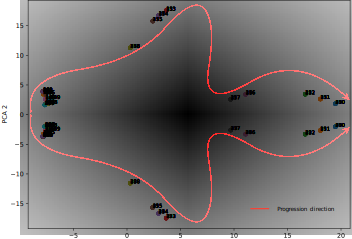
\includegraphics[width=0.8\linewidth]{figures/overcooked_figures/transition_pca.pdf}
  \caption{PCA of transition trajectories in Overcooked-AI}
  \label{fig:overcooked_pca}
\end{figure}

\

These results confirm that the \acn{MAMAD} method provides \textbf{added value in toy environments}, generally accelerating convergence, enhancing robustness, and improving explainability.
\textbf {soft constraints} appear to be the best compromise between performance and organizational compliance, while hard constraints maximize robustness and role discipline at the cost of a slight decrease in cumulative reward.
Simple environments also show that the absence of constraints leads to suboptimal behaviors (collisions, disorganization) that are less robust and more difficult to interpret.

\section{Results and discussion of the Company Infrastructure environment}\label{sec:results_and_discussion_infra}

\subsection*{Performance, convergence, and manual interventions}

\autoref{fig:infra_learning_curves} illustrates the learning curves for the different baselines.
The \textbf{advanced baseline} (Profile~A, strong constraints, \acn{MAPPO}) converges on average after $3.2 \times 10^4$ episodes, compared to $4.5 \times 10^4$ for ablation without constraints (\acn{TRN-UNC}).
The \textquote{QMIX} and \textquote {COMA} show slower convergence ($\sim 5.0 \times 10^4$ episodes), but achieve comparable rewards.

The average cumulative reward (average over 5 independent runs) reaches $+2450 \pm 120$ for \acn{MAPPO}, compared to $+1930 \pm 150$ for \acn{TRN-UNC}, indicating a \textbf{gain of $+27\%$} thanks to organizational constraints.

\begin{figure} [h!]
  \centering
  \includegraphics[width=0.75\linewidth]{figures/results_infra_learning.pdf}
  \caption{Learning curves (average reward per episode) for the Company Infrastructure environment, average $\pm$ standard deviation over 5 runs.}
  \label{fig:infra_learning_curves}
\end{figure}

In the Company Infrastructure environment, the average number of manual interventions required is 1 to 3 refinement cycles (i.e., 3 to 6 hours in total) to obtain an SMA whose performance is equivalent to that of a solution designed and implemented entirely manually, which generally requires more than a day's work. This represents a significant reduction in human intervention, estimated at between 15 and 25\%.

\subsection*{Robustness and adaptation}

Under disturbed scenarios (simultaneous attacks, intensive lateral movement, injected false positives), the \textbf{robustness score} (disturbed/nominal performance ratio) reaches $0.81$ for \acn{MAPPO} with strong constraints, compared to $0.63$ for \acn{TRN-UNC}.
The standard deviation of rewards is reduced ($\sigma = 140$ versus $220$), showing better inter-run stability. This may seem contradictory if we take into account the fact that constraints can also limit exploration and adaptation and thus reduce the ability to adapt to new scenarios. Nevertheless, in this specific case, it should be noted that there is a potential bias in that the organizational constraints were designed to cover a wide range of possible situations, which allowed the agents to develop robust strategies while remaining within the framework of the defined roles and missions.
On the other hand, soft constraints ($0.5$) offer an interesting compromise with a robustness score of $0.76$ and a slightly higher cumulative reward ($+2520$) thanks to greater freedom of exploration.

\subsection*{Constraint compliance and organizational control}

The \textbf{constraint violation rate} is zero (0.\%) in hard constraint mode, 4.3\% in soft mode, and 21.7\% without strong constraints (zero constraint hardness).
These results confirm the effectiveness of action masking.
However, there is an inverse correlation with cumulative reward: too many constraints can slow down initial learning, although the final plateau remains higher.

\subsection*{Organizational explainability}

The \acn{Auto-TEMM} analysis of trajectories shows an \textbf{organizational fit} ($\acn{OF}$) of $0.84$ for \acn{MAPPO} with strong constraints, compared to $0.67$ for \acn{TRN-UNC} .
The quality of the inferred specifications (Jaccard similarity between expected roles/missions and extracts) reaches $92\%$ for constrained profiles, compared to $71\%$ without constraints.
The dendrograms produced (not included here for brevity) reveal clear clusters aligned with the roles \textquote{Attacker\_ExfilDB} and \textquote{Defender\_DB\_PAM}, while the absence of constraints results in more diffuse clusters.

\subsection*{Comparative summary}

\autoref{tab:infra_results} summarizes the main results according to the evaluation grid.

\begin{table}[h!]
  \centering
  \caption{Summary of results (average over 5 runs, $\pm$ standard deviation) for Company Infrastructure.}
  \label{tab:infra_results}
  \renewcommand{\arraystretch}{1.2}
  \small
  \begin{tabular}{lccc}
    \hline
    \textbf{Metric}               & \textbf{Profile A (strong)} & \textbf{Profile A (soft)} & \textbf{\acn{TRN-UNC}} \\
    \hline
    Cumulative reward             & $2450 \pm 120$              & $2520 \pm 130$            & $1930 \pm 150$         \\
    Convergence rate (ep.)        & $32,000$                    & $29,500$                  & $45,000$               \\
    Robustness score              & $0.81$                      & $0.76$                    & $0.63$                 \\
    Standard deviation of rewards & $140$                       & $160$                     & $220$                  \\
    Constraint violations         & $0.0\%$                     & $4.3\%$                   & $21.7\%$               \\
    Organizational fit (\acn{OF}) & $0.84$                      & $0.79$                    & $0.67$                 \\
    Inferred specifications       & $92\%$                      & $88\%$                    & $71\%$                 \\
    \hline
  \end{tabular}
\end{table}

\

The results confirm that integrating \textbf{organizational constraints} (MOISE+ \allowbreak MARL) significantly improves the robustness, stability, and explainability of learned policies.
Nevertheless, hard constraints can slow convergence and slightly reduce the final cumulative reward compared to soft constraints, which offer an interesting compromise between performance and role compliance.
The absence of constraints leads to less robust and more difficult to interpret policies, which would limit their relevance in a real cyberdefense setting.


\section{Results and discussion of the Kubernetes Microservices environment}\label{sec:results_and_discussion_ms}

\subsection* {Summary of QoS performance, convergence, and manual interventions}

\autoref{fig:k8s_learning_curves} shows the learning curves (normalized overall QoS reward, moving average over $20$ episodes) for the main profiles.
Profile A (strong constraints, MAPPO) converges in $2.6 \times 10^4$ episodes (change-point plateau detection), compared to $3.9 \times 10^4$ for the TRN-UNC ablation.
The \textquote{MADDPG} and \textquote{QMIX} variants converge at $3.1\times 10^4$ and $3.5\times 10^4$ episodes, respectively.
Over $5$ independent runs, the final reward reaches $+0.91 \pm 0.03$ (normalized) for \acn{MAPPO}, $+0.88 \pm 0.04$ (strong), and $+0.79 \pm 0.05$ without constraints.

\begin{figure}[h!]
  \centering
  \includegraphics[width=0.75\linewidth]{figures/results_k8s_learning.pdf}
  \ caption[Learning curves (normalized QoS reward) for Kubernetes Microservices]{Learning curves (normalized QoS reward) for Kubernetes Microservices, average $\pm$ standard deviation over 5 runs.}
  \label{fig:k8s_learning_curves}
\end{figure}

Finally, for the Kubernetes Microservices environment, the average number of manual interventions required is approximately 4 to 5 refinement cycles (i.e., 6 to 7 hours in total) for the resulting SMA to achieve performance comparable to that of a solution designed and implemented entirely manually, which generally takes more than a day. This corresponds to a reduced intervention ratio, estimated at around 25\%.

\subsection*{QoS indicators under nominal conditions}

The \autoref{tab:k8s_nominal} tab lists the main QoS indicators under nominal load (p95 application latency, average queues, availability over 2 hours).
\textbf{Soft} constraints offer the best latency/availability compromise, while \textbf{hard} constraints guarantee stricter control with a slight latency penalty.

\begin{table}[h!]
  \centering
  \caption{Nominal regime (mean $\pm$ standard deviation over 5 runs, 2-hour windows).}
  \label{tab:k8s_nominal}
  \renewcommand{\arraystretch}{1.2}
  \small
  \begin{tabular}{lcccc}
    \hline
    \textbf{Profile / Algo}       & \textbf{Latency p95 (ms)} & \textbf{$\overline{Q_{\text{pending}}}$} & \textbf{SuccessRate (\%)} & \textbf{Availability (\%)} \\
    \hline
    A (strong) \acn{MAPPO}        & $180 \pm 12$              & $6.1 \pm 0.8$                            & $99.1 \pm 0.3$            & $99.96 \pm 0.02$           \\
    A (soft) \acn{MAPPO}          & $\mathbf{168 \pm 10}$     & $\mathbf{5.3 \pm 0.7}$                   & $\mathbf{99.3 \pm 0.2}$   & $\mathbf{99.97 \pm 0.01}$  \\
    À (\acn{TRN-UNC}) \acn{MAPPO} & $216 \pm 17$              & $8.4 \pm 1.1$                            & $98.5 \pm 0.4$            & $99.92 \pm 0.03$           \\
    \hdashline
    B (\acn{ANL-MAN}) \acn{COMA}  & $191 \pm 14$              & $6.8 \pm 0.9$                            & $99.0 \pm 0.3$            & $99.95 \pm 0.02$           \\
    \hdashline
    C (manual) \acn{HPA}          & $310 \pm 24$              & $14.2 \pm 1.9$                           & $97.6 \pm 0.8$            & $99.20 \pm 0.10$           \\
    \hline
  \end{tabular}
\end{table}

\subsection* {Robustness to disruptions}

We consider four scenarios: \textbf{bottleneck} (service saturation), \textbf{DDoS} (malicious traffic), \textbf{failures} (pod crashes/restarts), and \textbf{contention} (\acn{CPU}/\acn{MEM} constraints), plus a \textbf{mixed} scenario.
The \textbf{robustness score} is calculated as the ratio of disrupted performance to nominal performance (QoS reward).
\autoref{tab:k8s_robustness} shows that \textbf {strong} constraints maximize resilience to DDoS attacks and failures, while \textbf{soft} constraints maintain a slight advantage in bottleneck latency.

\begin{table}[h!]
  \centering
  \caption{Robustness per scenario (average over 5 runs).}
  \label{tab:k8s_robustness}
  \renewcommand{\arraystretch}{1.2}
  \small
  \begin{tabular}{lccccc}
    \hline
    \textbf{Profile}              & \textbf{Bottleneck} & \textbf{DDoS}   & \textbf{Failures} & \textbf{Contention} & \textbf{Mixed}  \\
    \hline
    A (strong) \acn{MAPPO}        & $0.84$              & $\mathbf{0.86}$ & $\mathbf{0.88}$   & $0.83$              & $\mathbf{0.85}$ \\
    A (soft) \acn{MAPPO}          & $\mathbf{0.86}$     & $0.82$          & $0.84$            & $\mathbf {0.85}$    & $0.83$          \\
    A (\acn{TRN-UNC}) \acn{MAPPO} & $0.73$              & $0.69$          & $0.71$            & $0.72$              & $0.68$          \\
    \acn{HPA}                     & $0.64$              & $0.58$          & $0.61$            & $0.62$              & $0.57$          \\
    \hline
  \end{tabular}
\end{table}

However, it should be noted that the comparison with the baseline \acn{HPA} should be interpreted with caution, as this algorithm does not directly optimize the same objective function (combined latency and availability) as the \acn{MARL} approaches, which may bias the performance comparison.

\subsection*{Recovery time and action discipline}

Under DDoS, the \textbf{recovery time} (return to $L_{\text{avg}}<200$ ms) is $3.7 \pm 0.6$ min for \acn{MAPPO} compared to $5.2 \pm 0.8$ min (soft) and $7.9 \pm 1.1$ min (\acn{TRN-UNC}).
The \textbf{rate of guardrail violations} (contradictory actions between roles, e.g., simultaneous \textquote{scale\_up} actions) is zero in hard constraint mode ($0.0\%$), $3.1\%$ in soft mode, and $18.4\%$ without hard constraints (zero constraint hardness).
The \textbf{inter-run standard deviation} on reward is reduced with constraints ($\sigma=0.028$ hard, $0.031$ soft) vs $0.049$ (\acn{TRN-UNC}), highlighting increased stability. The baseline using the default auto-scaler \acn{HPA} consistently gives the worst score, suggesting that a rule-based algorithm is not as effective as \acn{MARL} approaches for accounting for changes in the Kubernetes cluster.

\subsection* {Digital twin accuracy (simulation/actual deviation)}

The digital twin trains policies offline before transfer.
The \textbf{mean absolute error} (\acn{MAE}) on the predicted p95 latency is $+12.7$~ms (bottleneck), $+18.4$~ms (DDoS), $+15.1$ ms (outages), and $+21.3$ ms (mixed), representing a \textbf{relative error} of $6$–$9\% $.
The divergence on $\overline{Q_{\text{pending}}}$ remains $<1.7$ requests on average.
After fine-tuning on recent traces (one iteration), the MAE on p95 drops by $\sim 28\%$ (DDoS).

\subsection*{Organizational explainability}

\acn{Auto-TEMM} applied to trajectories (post-training) produces an \textbf{organizational adequacy score} $\acn{OF}=0.86$ (strong constraints) , $0.83$ (soft) and $0.71$ (\acn{TRN-UNC}).
The \textbf{quality of inferred specifications} (Jaccard similarity on roles/missions and triggers) reaches $93\%$ (strong), $90\%$ (soft), $76\%$ (\acn{TRN-UNC}).
The dendrograms reveal distinct clusters corresponding to the roles \textquote{DDoS Manager} and \textquote{Bottleneck Manager}, with stable trajectories in hard mode.

\subsection*{Summary comparison}

\begin{table}[h!]
  \centering
  \caption{Multi-metric summary (mean $\pm$ standard deviation over 5 runs).}
  \label{tab:k8s_summary}
  \renewcommand{\arraystretch}{1.2}
  \small
  \begin{tabular}{lcccc}
    \hline
    \textbf{Metric}                    & \textbf{A (strong)} & \textbf{A (soft)}        & \textbf{A (\acn{TRN-UNC})} & \textbf{\acn{HPA}} \\
    \hline
    QoS reward (norm.)                 & $0.88 \pm 0.04$     & $\mathbf{0.91 \pm 0.03}$ & $0.79 \pm 0.05$            & $0.66 \pm 0.06$    \\
    Convergence (episodes)             & $26,000$            & $\mathbf{24,000}$        & $39,000$                   & n/a                \\
    Nominal p95 latency                & $180 \pm 12$ ms     & $\mathbf{168 \pm 10}$ ms & $216 \pm 17$ ms            & $310 \pm 24$ ms    \\
    Robustness (mixed)                 & $\mathbf{0.85} $    & $0.83$                   & $0.68$                     & $0.57$             \\
    Constraint violations              & $\mathbf{0.0\%}$    & $3.1\%$                  & $18.4\%$                   & n/a                \\
    Organizational adequacy (\acn{OF}) & $\mathbf{0.86}$     & $0.83$                   & $0.71$                     & n/a                \\
    \hline
  \end{tabular}
\end{table}

\

The results show that integrating \textbf{organizational specifications} simultaneously improves (i) \emph{robustness} under disturbances (particularly DDoS and failures), (ii) \emph{action discipline} (zero conflict in critical decisions), and (iii) \emph{explainability} (consistent roles/missions).
Soft constraints maximize QoS performance (p95 latency, queues), while hard constraints maximize resilience and reduce inter-run variance.
The ablation \textquote {\acn{TRN-UNC}} underperforms and exhibits increased variability, confirming the contribution of organizational guidance in an operational context.
Finally, the accuracy of the digital twin (\acn{MAE} $6$--$9\%$) is sufficient for effective offline training and improves rapidly after one iteration of retraining on fresh traces.


\section{Results and discussion of the Drone Swarm environment}\label{sec:results_and_discussion_drone_swarm}

\subsection*{Summary of performance, convergence, and manual interventions}

\autoref{fig:drone_learning_curves} illustrates the learning curves (normalized reward) on the drone swarm (18 nodes).
Profile A (strong constraints, \acn{MAPPO}) converges in $3.1\times 10^4$ episodes, compared to $4.7\times 10^4$ for the ablation \textquote{\acn{TRN-UNC}}.
The variants \acn {MADDPG} and \acn{QMIX} variants reach $3.6\times 10^4$ and $4.2\times 10^4$ episodes, respectively.
In steady state, the average normalized rewards are $+0.87 \pm 0.04$ (\acn{MAPPO} strong), $+0.89 \pm 0.03$ (soft), and $+0.72 \pm 0.07$ without constraints.

\begin{figure}[h!]
  \centering
  \includegraphics[width=0.75\linewidth]{figures/results_drone_learning.pdf}
  \caption[Learning curves (normalized reward) for Drone Swarm]{Learning curves (normalized reward) for Drone Swarm, mean $\pm$ standard deviation over 5 runs.}
  \label{fig:drone_learning_curves}
\end{figure}

For the Drone Swarm environment, the average number of manual interventions required is approximately 2 to 3 refinement cycles (i.e., 4 to 5 hours in total) for the resulting SMA to achieve performance comparable to that of a solution designed and implemented entirely manually, which typically takes more than a day. This corresponds to a reduced intervention ratio, estimated at around 20\%.


\subsection*{Indicators in nominal operation}

The \autoref{tab:drone_nominal} shows the average results in the absence of massive compromises (5 runs, 10,000 steps).
Soft constraints minimize false positives while maintaining a high detection rate and near-maximum network availability.
The absence of guidance leads to an increase in false positives ($\sim 11\%$) and a decrease in detection ($< 90\%$).

\begin{table}[h!]
  \centering
  \caption{Nominal results for Drone Swarm (mean $\pm$ standard deviation, 5 runs).}
  \label{tab:drone_nominal}
  \renewcommand{\arraystretch}{1.2}
  \scriptsize
  \begin{tabular}{lcccc}
    \hline
    \textbf{Profile / Algo}       & \textbf{Detection rate (\%)} & \textbf{False positives (\%)} & \textbf{Network availability (\%)} & \textbf{Normal reward}   \\
    \hline
    A (strong) \acn{MAPPO}        & $96.8 \pm 0.7$               & $3.1 \pm 0.5$                 & $99.2 \pm 0.3$                     & $0.87 \pm 0.04$          \\
    A (soft) \acn{MAPPO}          & $\mathbf{97.3 \pm 0.6}$      & $\mathbf{2.7 \pm 0.4}$        & $\mathbf{99.4 \pm 0.2}$            & $\mathbf{0.89 \pm 0.03}$ \\
    À (\acn{TRN-UNC}) \acn{MAPPO} & $88.5 \pm 1.2$               & $11.2 \pm 1.6$                & $97.9 \pm 0.6$                     & $0.72 \pm 0.07$          \\
    \hdashline
    B (\acn{ANL-MAN}) \acn{COMA}  & $95.2 \pm 0.9$               & $4.5 \pm 0.8$                 & $99.0 \pm 0.3$                     & $0.85 \pm 0.04$          \\
    \hdashline
    C (manual) \acn{VDN}          & $91.7 \pm 1.4$               & $7.9 \pm 1.1$                 & $98.4 \pm 0.5$                     & $0.77 \pm 0.06$          \\
    \acn{IDS} rules (ref.)        & $83.4 \pm 2.1$               & $15.6 \pm 2.7$                & $96.1 \pm 1.0$                     & $0.61 \pm 0.08$          \\
    \acn{ML} sup. (ref.)          & $87.9 \pm 1.8$               & $12.3 \pm 1.9$                & $97.0 \pm 0.8$                     & $0.68 \pm 0.07$          \\
    \hline
  \end{tabular}
\end{table}

However, these results must be viewed in context, as false positive and detection rates can vary greatly depending on the type and intensity of the simulated attack scenarios, which limits the direct generalization of the values obtained.

\subsection*{Robustness to compromise}

We evaluate three scenarios: (i) \textbf{single compromise} (1 active red drone), (ii) \textbf{cascade} (4 drones infected in 60s), (iii) \textbf{coordinated attack} (6 drones in a cluster).
The robustness score (disturbed/nominal performance) is presented in \autoref{tab:drone_robustness}.
Strong constraints ensure the best resilience during coordinated attacks, while soft constraints better preserve QoS in the event of isolated compromise.

\begin{table}[h!]
  \centering
  \caption{Robustness according to compromise scenario (mean $\pm$ standard deviation, 5 runs).}
  \label{tab:drone_robustness}
  \renewcommand{\arraystretch}{1.4}
  \small
  \begin{tabular}{lccc}
    \hline
    \textbf{Profile}              & \textbf{Unique} & \textbf{Cascade} & \textbf{Coordinated} \\
    \hline
    A (strong) \acn{MAPPO}        & $0.91$          & $\mathbf{0.87}$  & $\mathbf{0.83}$      \\
    A (soft) \acn{MAPPO}          & $\mathbf{0.93}$ & $0.84$           & $0.79$               \\
    À (\acn{TRN-UNC}) \acn{MAPPO} & $0.79$          & $0.68$           & $0.61$               \\
    \acn{IDS} rules (ref.)        & $0.72$          & $0.55$           & $0.47$               \\
    \hline
  \end{tabular}
\end{table}

\subsection*{Reaction time and stability}

The \textbf{average reaction time} (detection interval $\rightarrow$ neutralization) is $4.1 \pm 0.7$ s for \acn{MAPPO}, $4.8 \pm 0.6$ s (soft) and $7.3 \pm 1.2$ s without constraints.
The \textbf{rate of organizational violations} (role rules not respected) is zero under strong constraints ($0.0\%$), $2.9\%$ in soft mode, and $>15\%$ without hard constraints.
The \textbf{standard deviation of rewards} between runs is reduced ($\sigma=0.032$ strong, $0.037$ soft, $0.065$ without constraints).

\subsection*{Organizational explainability}

\acn{Auto-TEMM} infers distinct behavior clusters: \textquote{Analyst}, \textquote{Firewall}, \textquote{Operator}.
The \textbf{consistency score} reaches $0.84$ (strong) and $0.82$ (soft).
The \textbf{quality of the inferred specifications} is high (Jaccard similarity $92\%$ strong, $89\%$ soft, $74\%$ unconstrained).
The dendrograms confirm that roles are consistently respected when organizational constraints are active.

\subsection*{Summary comparison}

\begin{table}[h!]
\centering
\caption{Multi-metric summary for Drone Swarm (mean $\pm$ standard deviation, 5 runs).}
\label{tab:drone_summary}
\renewcommand{\arraystretch}{1.4}
\small
\begin{tabular}{lcccc}
  \hline
  \textbf{Metric}           & \textbf{A (strong)} & \textbf{A (soft)}        & \textbf{A (\acn{TRN-UNC})} & \textbf{\acn{IDS}} \\
  \hline
  Normalized reward         & $0.87 \pm 0.04$     & $\mathbf{0.89 \pm 0.03}$ & $0.72 \pm 0.07$            & $0.61 \pm 0.08$    \\
  Convergence (episodes)    & $31,000$            & $\mathbf{29,000}$        & $47,000$                   & n/a                \\
  Detection (\%)            & $96.8$              & $\mathbf{97.3}$          & $88.5$                     & $83.4$             \\
  False positives (\%)      & $3.1$               & $\mathbf{2.7}$           & $11.2$                     & $15.6$             \\
  Coord. robustness         & $\mathbf{0.83}$     & $0.79$                   & $0.61$                     & $0.47$             \\
  Organizational violations & $\mathbf{0.0\%}$    & $2.9\%$                  & $16.2\%$                   & n/a                \\
  Consistency (\acn{TEMM})  & $\mathbf{0.84}$     & $0.82$                   & n/a                        & n/a                \\
  \hline
\end{tabular}
\end {table}

\

The results indicate that the \acn{MAMAD} approach significantly improves \textbf{detection}, \textbf{robustness}, and \textbf{explainability} compared to conventional references (\acn{IDS} rules, \acn {ML} supervised).
Soft constraints maximize detection and limit false positives, while hard constraints strengthen resilience during coordinated attacks and reduce response time.
Ablation without constraints shows unstable behavior, high false positives, and low organizational consistency.
Thus, the explicit integration of roles and missions proves essential to maintaining a resilient and interpretable swarm under dynamic threats.


\section{Comparative discussion of results}

\subsection{Coverage of criteria by the method}

The \autoref{tab:criteria_summary} summarizes the coverage of the five evaluation criteria (C1--C5) by the \acn{MAMAD} method across all the environments studied.
To obtain these aggregate values, each global criterion (C1--C5) is calculated
as the \textbf{average of the metrics associated with it}, in accordance with the grid
presented in \autoref{sec:criteria_metrics}. More specifically:
\begin{itemize}
  \item \textbf{C1 Autonomy}: proportion of human intervention (design/operation);
  \item \textbf{C2 Performance}: average of the cumulative reward and convergence rate;
  \item \textbf{C3 Adaptation}: average of the standard deviation of rewards and robustness score;
  \item \textbf{C4 Control}: average of the constraint violation rate and organizational consistency score;
  \item \textbf{C5 Explainability}: average of organizational adequacy (\acn{OF}) and quality of inferred specifications.
\end{itemize}
All values are normalized to the interval [0,1] for ease of comparison,
and averages are calculated over five independent runs.
Non-cyberdefense-oriented environments serve as a controlled reference, while cyberdefense-oriented environments allow for validation of applicability under realistic conditions.

\begin{table}[h!]
  \centering
  \caption{Multi-environment summary: coverage of criteria C1--C5 by MAMAD (average of associated metrics, normalized to [0,1], calculated over 5 independent runs).}
  \label{tab:criteria_summary}
  \renewcommand{\arraystretch}{1.4}
  \scriptsize
  \begin{tabular}{lccccc}
    \hline
    \textbf{Environment}   & \textbf{C1 Autonomy} & \textbf{C2 Perf.} & \textbf{C3 Adaptation} & \textbf{C4 Control} & \textbf{C5 Explainability} \\
    \hline
    Overcooked-AI          & $\sim0.20$           & $0.82$            & $0.80$                 & $0.75$              & $0.72$                     \\
    Predator-Prey          & $\sim0.20$           & $0.79$            & $0.77$                 & $0.73$              & $0.69$                     \\
    Warehouse Management   & $\sim0.20$           & $0.85$            & $0.82$                 & $0.77$              & $0.76$                     \\
    Company Infrastructure & $\sim0.25$           & $0.88$            & $0.83$                 & $0.85$              & $0.81$                     \\
    Microservices K8s      & $0.25$               & $0.91$            & $0.86$                 & $0.88$              & $0.83$                     \\
    Drone Swarm            & $\sim0.20$           & $0.89$            & $0.84$                 & $0.86$              & $0.82$                     \\
    \hdashline
    \textbf{Average}       & $0.21$               & $0.86$            & $0.82$                 & $0.81$              & $0.77$                     \\
    \hline
  \end{tabular}
\end{table}

\subsection{Critical analysis}

The results highlight several key points:
\begin{itemize}
\item \textbf{Performance (C2)} and \textbf{adaptation (C3)} are systematically improved by the use of organizational constraints (soft or strong), particularly in complex environments (Kubernetes, Drone Swarm).
.
\item \textbf{Control (C4)} benefits most from strong constraints, which ensure strict compliance with roles and missions, sometimes at the cost of a slight decrease in performance.
\item \textbf{Explainability (C5)} is generally satisfactory ($\sim 0.8$). More chaotic environments (Predator-Prey, Overcooked) lead to less stable organizational inferences.
\item \textbf{Autonomy (C1)} achieves scores showing that in operational environments (Company Infrastructure, Microservices, Drone Swarm), the complete \textbf{MOD}–\textbf{TRN}–\textbf{ANL}–\textbf{TRF} loop reduces human intervention by around 20\%.
\end {itemize}

\subsection{Potential biases and limitations}

Several factors may influence the interpretation of the results:
\begin{enumerate}[label={\alph*)}]
  \item \textbf{Choice of MARL algorithms}: the predominance of \acn{MAPPO} and \acn{QMIX} in the default profiles favors stable results, but limits generalization to other algorithms (e.g., multi-agent \acparen{DQN}).
  \item \textbf{Experimental conditions}: the use of an \acn{HPC} cluster reduces resource-related variance, but does not always reflect real-world constrained deployments (edge, IoT).
  \item \textbf{Constraint design}: the definition of roles and missions directly influences control and explainability (excessive strictness can bias comparisons).
  \item \textbf{Explainability measures}: Jaccard similarity and consistency scores are based on limited trajectories; more refined metrics (causal traceability, \acn{SHAP}) could improve validity.
\end{enumerate}

\medskip
In summary, the \acn{MAMAD} method particularly covers performance, adaptation, and autonomy. The biases identified open up prospects for refining the evaluation (more algorithms, physical deployments, advanced metrics).

\section{Conclusion}

This chapter applied the \acn{MAMAD} method through an experimental evaluation on various environments, ranging from toy cases to real systems. The results highlight several strengths: accelerated convergence, improved robustness and stability of multi-agent policies, and increased explainability through the integration of organizational specifications. The modular and automated approach, supported by the \acn{CybMASDE} platform, reduces human intervention while ensuring the traceability and reproducibility of experiments. Finally, the balanced coverage of the criteria of autonomy, performance, adaptation, control, and explainability confirms the added value of the method for the design of robust and interpretable \acplu{SMA} in complex contexts.

\clearpage
\thispagestyle{empty}
\null
\newpage


\chapter*{Conclusion}
\addcontentsline{toc}{chapter}{\textbf{Conclusion}}

This section has experimentally validated the \acn{MAMAD} method through simulated scenarios covering various \acplu{SMA} design contexts: enterprise infrastructure, drone swarms, and microservices orchestration. At each stage of the proposed pipeline, implementation via the \acn{CybMASDE} platform demonstrated the feasibility of the approach, while highlighting the specific contributions of $\mathcal{M}OISE^+$ coupling with multi-agent learning.

The results obtained show significant gains in terms of autonomy, resilience, and organizational compliance of agents. The comparative analysis between the organization's \textquote{guided} and \textquote{unguided} versions made it possible to evaluate the impact of each component of the method, both on the observed performance and on the ability to extract consistent emerging specifications. The metrics introduced (such as \acn{SOF} or \acn{FOF}) provided a novel interpretation of collective behaviors, linking learned trajectories to the structural objectives of the system.

Despite these encouraging results, several limitations were identified: dependence on simulated environments, partial coverage of application contexts, and the need for significant computational resources. These elements will be discussed in more detail in the last part of this manuscript, which offers a reflective review of the entire process undertaken.

\vspace{1em}

\noindent
In the following, we will summarize the contributions, discuss the limitations of the method, and open up perspectives on its future extension, both in research and in application.

% ===============ttt



\subsection{Description of the experimental protocol instance}

\paragraph{1. Initial configuration}

We operate \emph{on the actual cluster} (no command line simulation playing the role of the \textquote{actual environment}). The cluster (\textbf{\acn{VM} 8~vCPU, 32 GB \acn{RAM}, 1 Gbps}) hosts the e-commerce application (4 microservices in a chain). Telemetry is collected by \textit{Prometheus} and visualized via \textit{Grafana}. \textquote{CybMASDE}/\textquote{KARMA} interfaces with the Kubernetes \acn{API} to \textit {observe} the status and \textit{act} (scaling, isolation, restart). A \textbf{digital twin} is built from the traces to train the policies offline, which are then \textbf{transferred} and \textit{closed in a loop} on the cluster (iterative learning by refreshing traces).

\begin{figure}[h!]
  \centering
  \resizebox{\textwidth}{!}{%
    


\tikzset{every picture/.style={line width=0.75pt}} %set default line width to 0.75pt        

\begin{tikzpicture}[x=0.75pt,y=0.75pt,yscale=-1.2,xscale=1.2]
%uncomment if require: \path (0,1414); %set diagram left start at 0, and has height of 1414

%Straight Lines [id:da5609883377896374] 
\draw [color={rgb, 255:red, 74; green, 144; blue, 226 }  ,draw opacity=1 ][line width=2.25]    (317.22,111.13) -- (360.07,111.13) ;
\draw [shift={(365.07,111.13)}, rotate = 180] [fill={rgb, 255:red, 74; green, 144; blue, 226 }  ,fill opacity=1 ][line width=0.08]  [draw opacity=0] (5.72,-2.75) -- (0,0) -- (5.72,2.75) -- cycle    ;
%Image [id:dp9396292457736715] 
\draw (106.77,60.95) node  {\includegraphics[width=18.66pt,height=18.36pt]{figures/karma_architecture/pod.png}};
%Image [id:dp3874378335758297] 
\draw (145.86,60.95) node  {\includegraphics[width=18.66pt,height=18.36pt]{figures/karma_architecture/pod.png}};
%Shape: Rectangle [id:dp4562827234223257] 
\draw  [color={rgb, 255:red, 74; green, 144; blue, 226 }  ,draw opacity=1 ][line width=1.5]  (89,28.36) .. controls (89,25.6) and (91.24,23.36) .. (94,23.36) -- (255,23.36) .. controls (257.76,23.36) and (260,25.6) .. (260,28.36) -- (260,132) .. controls (260,134.76) and (257.76,137) .. (255,137) -- (94,137) .. controls (91.24,137) and (89,134.76) .. (89,132) -- cycle ;
%Image [id:dp9455935833751838] 
\draw (172.5,16.24) node  {\includegraphics[width=18.66pt,height=18.36pt]{figures/karma_architecture/kubernetes.png}};
%Shape: Rectangle [id:dp9564725691593288] 
\draw  [color={rgb, 255:red, 74; green, 144; blue, 226 }  ,draw opacity=1 ][line width=1.5]  (92.55,50.21) .. controls (92.55,47.45) and (94.79,45.21) .. (97.55,45.21) -- (155.08,45.21) .. controls (157.84,45.21) and (160.08,47.45) .. (160.08,50.21) -- (160.08,70.81) .. controls (160.08,73.57) and (157.84,75.81) .. (155.08,75.81) -- (97.55,75.81) .. controls (94.79,75.81) and (92.55,73.57) .. (92.55,70.81) -- cycle ;
%Image [id:dp9120856447688912] 
\draw (126.32,39.97) node  {\includegraphics[width=18.66pt,height=18.36pt]{figures/karma_architecture/node.png}};
%Image [id:dp5738167237736518] 
\draw (106.77,119.52) node  {\includegraphics[width=18.66pt,height=18.36pt]{figures/karma_architecture/pod.png}};
%Image [id:dp2199681121060142] 
\draw (145.86,119.52) node  {\includegraphics[width=18.66pt,height=18.36pt]{figures/karma_architecture/pod.png}};
%Shape: Rectangle [id:dp12159705904547402] 
\draw  [color={rgb, 255:red, 74; green, 144; blue, 226 }  ,draw opacity=1 ][line width=1.5]  (92.55,108.78) .. controls (92.55,106.02) and (94.79,103.78) .. (97.55,103.78) -- (155.08,103.78) .. controls (157.84,103.78) and (160.08,106.02) .. (160.08,108.78) -- (160.08,129.38) .. controls (160.08,132.14) and (157.84,134.38) .. (155.08,134.38) -- (97.55,134.38) .. controls (94.79,134.38) and (92.55,132.14) .. (92.55,129.38) -- cycle ;
%Image [id:dp37768653229718074] 
\draw (126.32,98.54) node  {\includegraphics[width=18.66pt,height=18.36pt]{figures/karma_architecture/node.png}};
%Shape: Rectangle [id:dp20840815212238661] 
\draw  [color={rgb, 255:red, 74; green, 144; blue, 226 }  ,draw opacity=1 ][line width=1.5]  (264,28.36) .. controls (264,25.6) and (266.24,23.36) .. (269,23.36) -- (411.78,23.36) .. controls (414.54,23.36) and (416.78,25.6) .. (416.78,28.36) -- (416.78,132) .. controls (416.78,134.76) and (414.54,137) .. (411.78,137) -- (269,137) .. controls (266.24,137) and (264,134.76) .. (264,132) -- cycle ;
%Straight Lines [id:da9232180983272227] 
\draw [color={rgb, 255:red, 74; green, 144; blue, 226 }  ,draw opacity=1 ][line width=2.25]    (164,112) -- (201,112) ;
\draw [shift={(206,112)}, rotate = 180] [fill={rgb, 255:red, 74; green, 144; blue, 226 }  ,fill opacity=1 ][line width=0.08]  [draw opacity=0] (5.72,-2.75) -- (0,0) -- (5.72,2.75) -- cycle    ;
%Straight Lines [id:da6082715106712999] 
\draw [color={rgb, 255:red, 74; green, 144; blue, 226 }  ,draw opacity=1 ][line width=2.25]    (180,90.22) -- (167,90.22) ;
\draw [shift={(162,90.22)}, rotate = 360] [fill={rgb, 255:red, 74; green, 144; blue, 226 }  ,fill opacity=1 ][line width=0.08]  [draw opacity=0] (5.72,-2.75) -- (0,0) -- (5.72,2.75) -- cycle    ;
%Straight Lines [id:da30764510910060716] 
\draw [color={rgb, 255:red, 74; green, 144; blue, 226 }  ,draw opacity=1 ][line width=2.25]    (210,72) -- (199,72) ;
\draw [shift={(194,72)}, rotate = 360] [fill={rgb, 255:red, 74; green, 144; blue, 226 }  ,fill opacity=1 ][line width=0.08]  [draw opacity=0] (5.72,-2.75) -- (0,0) -- (5.72,2.75) -- cycle    ;
%Straight Lines [id:da5394403186779959] 
\draw [color={rgb, 255:red, 74; green, 144; blue, 226 }  ,draw opacity=1 ][line width=2.25]    (178,56.22) -- (167,56.22) ;
\draw [shift={(162,56.22)}, rotate = 360] [fill={rgb, 255:red, 74; green, 144; blue, 226 }  ,fill opacity=1 ][line width=0.08]  [draw opacity=0] (5.72,-2.75) -- (0,0) -- (5.72,2.75) -- cycle    ;
%Straight Lines [id:da6399475815904785] 
\draw [color={rgb, 255:red, 74; green, 144; blue, 226 }  ,draw opacity=1 ][line width=2.25]    (272,72) -- (235,72) ;
\draw [shift={(230,72)}, rotate = 360] [fill={rgb, 255:red, 74; green, 144; blue, 226 }  ,fill opacity=1 ][line width=0.08]  [draw opacity=0] (5.72,-2.75) -- (0,0) -- (5.72,2.75) -- cycle    ;
%Straight Lines [id:da24320102833940327] 
\draw [color={rgb, 255:red, 74; green, 144; blue, 226 }  ,draw opacity=1 ][line width=2.25]    (267,112) -- (230,112) ;
\draw [shift={(272,112)}, rotate = 180] [fill={rgb, 255:red, 74; green, 144; blue, 226 }  ,fill opacity=1 ][line width=0.08]  [draw opacity=0] (5.72,-2.75) -- (0,0) -- (5.72,2.75) -- cycle    ;
%Shape: Rectangle [id:dp9149123987409296] 
\draw  [color={rgb, 255:red, 255; green, 255; blue, 255 }  ,draw opacity=1 ][fill={rgb, 255:red, 255; green, 255; blue, 255 }  ,fill opacity=1 ] (328.83,106.67) -- (353.11,106.67) -- (353.11,114) -- (328.83,114) -- cycle ;
%Image [id:dp7127891043436136] 
\draw (341.68,109.47) node  {\includegraphics[width=14.57pt,height=15.21pt]{figures/karma_architecture/pettingzoo.png}};
%Straight Lines [id:da5757027637146572] 
\draw [color={rgb, 255:red, 74; green, 144; blue, 226 }  ,draw opacity=1 ][line width=2.25]    (357.9,41) -- (364.9,41) ;
\draw [shift={(352.9,41)}, rotate = 0] [fill={rgb, 255:red, 74; green, 144; blue, 226 }  ,fill opacity=1 ][line width=0.08]  [draw opacity=0] (5.72,-2.75) -- (0,0) -- (5.72,2.75) -- cycle    ;
%Straight Lines [id:da29364722138505184] 
\draw [color={rgb, 255:red, 74; green, 144; blue, 226 }  ,draw opacity=1 ][line width=2.25]    (390.99,97.77) -- (390.99,57.25) ;
\draw [shift={(390.99,52.25)}, rotate = 90] [fill={rgb, 255:red, 74; green, 144; blue, 226 }  ,fill opacity=1 ][line width=0.08]  [draw opacity=0] (5.72,-2.75) -- (0,0) -- (5.72,2.75) -- cycle    ;
%Straight Lines [id:da5470457469462804] 
\draw [color={rgb, 255:red, 74; green, 144; blue, 226 }  ,draw opacity=1 ][line width=2.25]    (390.9,71) -- (325.9,71) ;
\draw [shift={(320.9,71)}, rotate = 360] [fill={rgb, 255:red, 74; green, 144; blue, 226 }  ,fill opacity=1 ][line width=0.08]  [draw opacity=0] (5.72,-2.75) -- (0,0) -- (5.72,2.75) -- cycle    ;
%Shape: Rectangle [id:dp8476965567779329] 
\draw  [color={rgb, 255:red, 255; green, 255; blue, 255 }  ,draw opacity=1 ][fill={rgb, 255:red, 255; green, 255; blue, 255 }  ,fill opacity=1 ] (378.41,65.11) -- (397.83,65.11) -- (397.83,92) -- (378.41,92) -- cycle ;
%Shape: Smiley Face [id:dp8656850497140396] 
\draw  [fill={rgb, 255:red, 255; green, 255; blue, 255 }  ,fill opacity=1 ][line width=0.75]  (380.35,69.4) .. controls (380.35,67.3) and (382.09,65.6) .. (384.24,65.6) .. controls (386.38,65.6) and (388.12,67.3) .. (388.12,69.4) .. controls (388.12,71.5) and (386.38,73.2) .. (384.24,73.2) .. controls (382.09,73.2) and (380.35,71.5) .. (380.35,69.4) -- cycle ; \draw  [fill={rgb, 255:red, 255; green, 255; blue, 255 }  ,fill opacity=1 ][line width=0.75]  (382.53,68.11) .. controls (382.53,67.9) and (382.7,67.73) .. (382.92,67.73) .. controls (383.13,67.73) and (383.31,67.9) .. (383.31,68.11) .. controls (383.31,68.32) and (383.13,68.49) .. (382.92,68.49) .. controls (382.7,68.49) and (382.53,68.32) .. (382.53,68.11) -- cycle ; \draw  [fill={rgb, 255:red, 255; green, 255; blue, 255 }  ,fill opacity=1 ][line width=0.75]  (385.17,68.11) .. controls (385.17,67.9) and (385.34,67.73) .. (385.56,67.73) .. controls (385.77,67.73) and (385.95,67.9) .. (385.95,68.11) .. controls (385.95,68.32) and (385.77,68.49) .. (385.56,68.49) .. controls (385.34,68.49) and (385.17,68.32) .. (385.17,68.11) -- cycle ; \draw  [line width=0.75]  (382.29,70.92) .. controls (383.59,71.94) and (384.88,71.94) .. (386.18,70.92) ;
%Shape: Smiley Face [id:dp9163740789669144] 
\draw  [fill={rgb, 255:red, 255; green, 255; blue, 255 }  ,fill opacity=1 ][line width=0.75]  (392.01,69.4) .. controls (392.01,67.3) and (393.75,65.6) .. (395.89,65.6) .. controls (398.04,65.6) and (399.78,67.3) .. (399.78,69.4) .. controls (399.78,71.5) and (398.04,73.2) .. (395.89,73.2) .. controls (393.75,73.2) and (392.01,71.5) .. (392.01,69.4) -- cycle ; \draw  [fill={rgb, 255:red, 255; green, 255; blue, 255 }  ,fill opacity=1 ][line width=0.75]  (394.18,68.11) .. controls (394.18,67.9) and (394.36,67.73) .. (394.57,67.73) .. controls (394.79,67.73) and (394.96,67.9) .. (394.96,68.11) .. controls (394.96,68.32) and (394.79,68.49) .. (394.57,68.49) .. controls (394.36,68.49) and (394.18,68.32) .. (394.18,68.11) -- cycle ; \draw  [fill={rgb, 255:red, 255; green, 255; blue, 255 }  ,fill opacity=1 ][line width=0.75]  (396.82,68.11) .. controls (396.82,67.9) and (397,67.73) .. (397.21,67.73) .. controls (397.43,67.73) and (397.6,67.9) .. (397.6,68.11) .. controls (397.6,68.32) and (397.43,68.49) .. (397.21,68.49) .. controls (397,68.49) and (396.82,68.32) .. (396.82,68.11) -- cycle ; \draw  [line width=0.75]  (393.95,70.92) .. controls (395.24,71.94) and (396.54,71.94) .. (397.83,70.92) ;
%Shape: Smiley Face [id:dp8186451078369623] 
\draw  [fill={rgb, 255:red, 255; green, 255; blue, 255 }  ,fill opacity=1 ][line width=0.75]  (386.18,77.44) .. controls (386.18,75.34) and (387.92,73.64) .. (390.06,73.64) .. controls (392.21,73.64) and (393.95,75.34) .. (393.95,77.44) .. controls (393.95,79.54) and (392.21,81.24) .. (390.06,81.24) .. controls (387.92,81.24) and (386.18,79.54) .. (386.18,77.44) -- cycle ; \draw  [fill={rgb, 255:red, 255; green, 255; blue, 255 }  ,fill opacity=1 ][line width=0.75]  (388.36,76.15) .. controls (388.36,75.94) and (388.53,75.77) .. (388.74,75.77) .. controls (388.96,75.77) and (389.13,75.94) .. (389.13,76.15) .. controls (389.13,76.36) and (388.96,76.53) .. (388.74,76.53) .. controls (388.53,76.53) and (388.36,76.36) .. (388.36,76.15) -- cycle ; \draw  [fill={rgb, 255:red, 255; green, 255; blue, 255 }  ,fill opacity=1 ][line width=0.75]  (391,76.15) .. controls (391,75.94) and (391.17,75.77) .. (391.39,75.77) .. controls (391.6,75.77) and (391.77,75.94) .. (391.77,76.15) .. controls (391.77,76.36) and (391.6,76.53) .. (391.39,76.53) .. controls (391.17,76.53) and (391,76.36) .. (391,76.15) -- cycle ; \draw  [line width=0.75]  (388.12,78.96) .. controls (389.42,79.98) and (390.71,79.98) .. (392.01,78.96) ;
%Flowchart: Punched Tape [id:dp6020643269389074] 
\draw  [fill={rgb, 255:red, 255; green, 255; blue, 255 }  ,fill opacity=1 ] (313.9,33.81) .. controls (313.9,35.03) and (318.18,36.02) .. (323.45,36.02) .. controls (328.73,36.02) and (333,35.03) .. (333,33.81) .. controls (333,32.58) and (337.28,31.59) .. (342.55,31.59) .. controls (347.83,31.59) and (352.1,32.58) .. (352.1,33.81) -- (352.1,51.52) .. controls (352.1,50.3) and (347.83,49.31) .. (342.55,49.31) .. controls (337.28,49.31) and (333,50.3) .. (333,51.52) .. controls (333,52.75) and (328.73,53.74) .. (323.45,53.74) .. controls (318.18,53.74) and (313.9,52.75) .. (313.9,51.52) -- cycle ;
%Straight Lines [id:da950307097731951] 
\draw [line width=0.75]    (324.14,41.04) -- (341.9,41) ;
%Shape: Smiley Face [id:dp8914579811118104] 
\draw  [line width=0.75]  (320.58,40.88) .. controls (320.58,39.7) and (321.59,38.73) .. (322.85,38.73) .. controls (324.1,38.73) and (325.11,39.7) .. (325.11,40.88) .. controls (325.11,42.07) and (324.1,43.03) .. (322.85,43.03) .. controls (321.59,43.03) and (320.58,42.07) .. (320.58,40.88) -- cycle ; \draw  [line width=0.75]  (321.85,40.15) .. controls (321.85,40.03) and (321.95,39.94) .. (322.08,39.94) .. controls (322.2,39.94) and (322.3,40.03) .. (322.3,40.15) .. controls (322.3,40.27) and (322.2,40.37) .. (322.08,40.37) .. controls (321.95,40.37) and (321.85,40.27) .. (321.85,40.15) -- cycle ; \draw  [line width=0.75]  (323.39,40.15) .. controls (323.39,40.03) and (323.49,39.94) .. (323.62,39.94) .. controls (323.74,39.94) and (323.84,40.03) .. (323.84,40.15) .. controls (323.84,40.27) and (323.74,40.37) .. (323.62,40.37) .. controls (323.49,40.37) and (323.39,40.27) .. (323.39,40.15) -- cycle ; \draw  [line width=0.75]  (321.71,41.74) .. controls (322.47,42.31) and (323.22,42.31) .. (323.98,41.74) ;
%Shape: Smiley Face [id:dp07941198495535606] 
\draw  [line width=0.75]  (329.9,45.15) .. controls (329.9,43.96) and (330.92,43) .. (332.17,43) .. controls (333.42,43) and (334.44,43.96) .. (334.44,45.15) .. controls (334.44,46.33) and (333.42,47.29) .. (332.17,47.29) .. controls (330.92,47.29) and (329.9,46.33) .. (329.9,45.15) -- cycle ; \draw  [line width=0.75]  (331.17,44.42) .. controls (331.17,44.3) and (331.28,44.2) .. (331.4,44.2) .. controls (331.53,44.2) and (331.63,44.3) .. (331.63,44.42) .. controls (331.63,44.54) and (331.53,44.63) .. (331.4,44.63) .. controls (331.28,44.63) and (331.17,44.54) .. (331.17,44.42) -- cycle ; \draw  [line width=0.75]  (332.72,44.42) .. controls (332.72,44.3) and (332.82,44.2) .. (332.94,44.2) .. controls (333.07,44.2) and (333.17,44.3) .. (333.17,44.42) .. controls (333.17,44.54) and (333.07,44.63) .. (332.94,44.63) .. controls (332.82,44.63) and (332.72,44.54) .. (332.72,44.42) -- cycle ; \draw  [line width=0.75]  (331.04,46.01) .. controls (331.79,46.58) and (332.55,46.58) .. (333.3,46.01) ;
%Shape: Smiley Face [id:dp8353415903298282] 
\draw  [line width=0.75]  (341.9,40.85) .. controls (341.9,39.67) and (342.92,38.71) .. (344.17,38.71) .. controls (345.42,38.71) and (346.44,39.67) .. (346.44,40.85) .. controls (346.44,42.04) and (345.42,43) .. (344.17,43) .. controls (342.92,43) and (341.9,42.04) .. (341.9,40.85) -- cycle ; \draw  [line width=0.75]  (343.17,40.12) .. controls (343.17,40) and (343.28,39.91) .. (343.4,39.91) .. controls (343.53,39.91) and (343.63,40) .. (343.63,40.12) .. controls (343.63,40.24) and (343.53,40.34) .. (343.4,40.34) .. controls (343.28,40.34) and (343.17,40.24) .. (343.17,40.12) -- cycle ; \draw  [line width=0.75]  (344.72,40.12) .. controls (344.72,40) and (344.82,39.91) .. (344.94,39.91) .. controls (345.07,39.91) and (345.17,40) .. (345.17,40.12) .. controls (345.17,40.24) and (345.07,40.34) .. (344.94,40.34) .. controls (344.82,40.34) and (344.72,40.24) .. (344.72,40.12) -- cycle ; \draw  [line width=0.75]  (343.04,41.71) .. controls (343.79,42.28) and (344.55,42.28) .. (345.3,41.71) ;
%Straight Lines [id:da21936285199788075] 
\draw [line width=0.75]    (324.19,41.87) -- (329.9,45) ;
%Image [id:dp05694376090002984] 
\draw (218.44,70.24) node  {\includegraphics[width=18.66pt,height=18.36pt]{figures/karma_architecture/api.png}};
%Image [id:dp7747210194064744] 
\draw (186.74,54.54) node  {\includegraphics[width=18.66pt,height=18.36pt]{figures/karma_architecture/deploy.png}};
%Image [id:dp5268588430037433] 
\draw (186.74,87.76) node  {\includegraphics[width=18.66pt,height=18.36pt]{figures/karma_architecture/deploy.png}};
%Image [id:dp7447308292951857] 
\draw (218.44,111.76) node  {\includegraphics[width=18.66pt,height=18.36pt]{figures/karma_architecture/prometheus.png}};
%Shape: Rectangle [id:dp7837974954754439] 
\draw  [color={rgb, 255:red, 75; green, 101; blue, 225 }  ,draw opacity=1 ][fill={rgb, 255:red, 74; green, 144; blue, 226 }  ,fill opacity=1 ] (202.37,94.64) -- (208.29,94.64) -- (208.29,101.67) -- (202.37,101.67) -- cycle ;
%Shape: Rectangle [id:dp780870970882084] 
\draw  [color={rgb, 255:red, 75; green, 101; blue, 225 }  ,draw opacity=1 ][fill={rgb, 255:red, 74; green, 144; blue, 226 }  ,fill opacity=1 ] (286.37,126) -- (292.29,126) -- (292.29,133.03) -- (286.37,133.03) -- cycle ;

%Shape: Rectangle [id:dp7051683429553395] 
\draw  [color={rgb, 255:red, 75; green, 101; blue, 225 }  ,draw opacity=1 ][fill={rgb, 255:red, 74; green, 144; blue, 226 }  ,fill opacity=1 ] (397.37,124.64) -- (403.29,124.64) -- (403.29,131.67) -- (397.37,131.67) -- cycle ;

%Shape: Rectangle [id:dp5578959475333973] 
\draw  [color={rgb, 255:red, 75; green, 101; blue, 225 }  ,draw opacity=1 ][fill={rgb, 255:red, 74; green, 144; blue, 226 }  ,fill opacity=1 ] (368.37,54.64) -- (374.29,54.64) -- (374.29,61.67) -- (368.37,61.67) -- cycle ;

%Shape: Rectangle [id:dp2822949836407178] 
\draw  [color={rgb, 255:red, 75; green, 101; blue, 225 }  ,draw opacity=1 ][fill={rgb, 255:red, 74; green, 144; blue, 226 }  ,fill opacity=1 ] (324.37,78) -- (330.29,78) -- (330.29,85.03) -- (324.37,85.03) -- cycle ;

%Shape: Rectangle [id:dp9339299822588341] 
\draw  [color={rgb, 255:red, 75; green, 101; blue, 225 }  ,draw opacity=1 ][fill={rgb, 255:red, 74; green, 144; blue, 226 }  ,fill opacity=1 ] (205.37,48) -- (211.29,48) -- (211.29,55.03) -- (205.37,55.03) -- cycle ;



% Text Node
\draw (205.5,98.5) node  [font=\fontsize{0.33em}{0.4em}\selectfont,color={rgb, 255:red, 255; green, 255; blue, 255 }  ,opacity=1 ] [align=left] {1};
% Text Node
\draw (244,58.5) node  [font=\normalsize] [align=left] {{\tiny Scaling}};
\draw (244,64.5) node  [font=\normalsize] [align=left] {{\tiny actions}};
% Text Node
\draw (244,99.5) node  [font=\normalsize] [align=left] {{\tiny Metrics}};
\draw (244,105.5) node  [font=\normalsize] [align=left] {{\tiny data}};
% Text Node
\draw (344.5,36) node  [font=\fontsize{0.33em}{0.4em}\selectfont] [align=left] {\begin{minipage}[lt]{8.66pt}\setlength\topsep{0pt}
\begin{center}
{\fontsize{0.33em}{0.4em}\selectfont $\displaystyle \mathbf{\textcolor[rgb]{0.82,0.01,0.11}{\pi }\textcolor[rgb]{0.82,0.01,0.11}{_{3}}}$}
\end{center}

\end{minipage}};
% Text Node
\draw (341,46.5) node  [font=\fontsize{0.33em}{0.4em}\selectfont] [align=left] {\begin{minipage}[lt]{8.66pt}\setlength\topsep{0pt}
\begin{center}
{\fontsize{0.33em}{0.4em}\selectfont $\displaystyle \mathbf{\textcolor[rgb]{0.82,0.01,0.11}{\pi }\textcolor[rgb]{0.82,0.01,0.11}{_{2}}}$}
\end{center}

\end{minipage}};
% Text Node
\draw (320.9,48) node  [font=\fontsize{0.33em}{0.4em}\selectfont] [align=left] {\begin{minipage}[lt]{8.66pt}\setlength\topsep{0pt}
\begin{center}
{\fontsize{0.33em}{0.4em}\selectfont $\displaystyle \mathbf{\textcolor[rgb]{0.82,0.01,0.11}{\pi }\textcolor[rgb]{0.82,0.01,0.11}{_{1}}}$}
\end{center}

\end{minipage}};
% Text Node
\draw  [color={rgb, 255:red, 75; green, 101; blue, 225 }  ,draw opacity=1 ][fill={rgb, 255:red, 136; green, 197; blue, 246 }  ,fill opacity=1 ][line width=1.5]   (322.77,14.89) .. controls (322.77,13.78) and (323.67,12.89) .. (324.77,12.89) -- (355.77,12.89) .. controls (356.88,12.89) and (357.77,13.78) .. (357.77,14.89) -- (357.77,26.89) .. controls (357.77,27.99) and (356.88,28.89) .. (355.77,28.89) -- (324.77,28.89) .. controls (323.67,28.89) and (322.77,27.99) .. (322.77,26.89) -- cycle  ;
\draw (340.27,20.89) node  [font=\tiny] [align=left] {\begin{minipage}[lt]{21.5pt}\setlength\topsep{0pt}
\begin{center}
KARMA
\end{center}

\end{minipage}};
% Text Node
\draw (290,40.5) node  [font=\tiny] [align=left] {\begin{minipage}[lt]{27.24pt}\setlength\topsep{0pt}
\begin{center}
Organizational\\Analysis
\end{center}

\end{minipage}};
% Text Node
\draw (388,86.39) node  [font=\tiny] [align=left] {\begin{minipage}[lt]{43.42pt}\setlength\topsep{0pt}
\begin{center}
Trained policies
\end{center}

\end{minipage}};
% Text Node
\draw (344.13,127.35) node  [font=\tiny] [align=left] {\begin{minipage}[lt]{60.78pt}\setlength\topsep{0pt}
\begin{center}
PettingZoo environment
\end{center}

\end{minipage}};
% Text Node
\draw (218,127) node  [font=\tiny] [align=left] {\begin{minipage}[lt]{30.31pt}\setlength\topsep{0pt}
\begin{center}
Prometheus
\end{center}

\end{minipage}};
% Text Node
\draw  [color={rgb, 255:red, 75; green, 101; blue, 225 }  ,draw opacity=1 ][fill={rgb, 255:red, 136; green, 197; blue, 246 }  ,fill opacity=1 ][line width=1.5]   (272.9,62) .. controls (272.9,60.9) and (273.8,60) .. (274.9,60) -- (317.9,60) .. controls (319.01,60) and (319.9,60.9) .. (319.9,62) -- (319.9,83) .. controls (319.9,84.1) and (319.01,85) .. (317.9,85) -- (274.9,85) .. controls (273.8,85) and (272.9,84.1) .. (272.9,83) -- cycle  ;
\draw (296.4,72.5) node  [font=\tiny,color={rgb, 255:red, 0; green, 0; blue, 0 }  ,opacity=1 ] [align=left] {Transfer\\Component};
% Text Node
\draw  [color={rgb, 255:red, 75; green, 101; blue, 225 }  ,draw opacity=1 ][fill={rgb, 255:red, 136; green, 197; blue, 246 }  ,fill opacity=1 ][line width=1.5]   (365.88,29.46) .. controls (365.88,28.35) and (366.78,27.46) .. (367.88,27.46) -- (410.88,27.46) .. controls (411.99,27.46) and (412.88,28.35) .. (412.88,29.46) -- (412.88,50.46) .. controls (412.88,51.56) and (411.99,52.46) .. (410.88,52.46) -- (367.88,52.46) .. controls (366.78,52.46) and (365.88,51.56) .. (365.88,50.46) -- cycle  ;
\draw (389.38,39.96) node  [font=\tiny,color={rgb, 255:red, 0; green, 0; blue, 0 }  ,opacity=1 ] [align=left] {Analyzing\\Component};
% Text Node
\draw  [color={rgb, 255:red, 75; green, 101; blue, 225 }  ,draw opacity=1 ][fill={rgb, 255:red, 136; green, 197; blue, 246 }  ,fill opacity=1 ][line width=1.5]   (365.88,98.24) .. controls (365.88,97.13) and (366.78,96.24) .. (367.88,96.24) -- (410.88,96.24) .. controls (411.99,96.24) and (412.88,97.13) .. (412.88,98.24) -- (412.88,119.24) .. controls (412.88,120.34) and (411.99,121.24) .. (410.88,121.24) -- (367.88,121.24) .. controls (366.78,121.24) and (365.88,120.34) .. (365.88,119.24) -- cycle  ;
\draw (389.38,108.74) node  [font=\tiny,color={rgb, 255:red, 0; green, 0; blue, 0 }  ,opacity=1 ] [align=left] {Training\\Component};
% Text Node
\draw (172.5,33.36) node  [font=\tiny] [align=left] {\begin{minipage}[lt]{16.92pt}\setlength\topsep{0pt}
\begin{center}
Cluster
\end{center}

\end{minipage}};
% Text Node
\draw  [color={rgb, 255:red, 75; green, 101; blue, 225 }  ,draw opacity=1 ][fill={rgb, 255:red, 136; green, 197; blue, 246 }  ,fill opacity=1 ][line width=1.5]   (272.9,99) .. controls (272.9,97.9) and (273.8,97) .. (274.9,97) -- (317.9,97) .. controls (319.01,97) and (319.9,97.9) .. (319.9,99) -- (319.9,120) .. controls (319.9,121.1) and (319.01,122) .. (317.9,122) -- (274.9,122) .. controls (273.8,122) and (272.9,121.1) .. (272.9,120) -- cycle  ;
\draw (296.4,109.5) node  [font=\tiny,color={rgb, 255:red, 0; green, 0; blue, 0 }  ,opacity=1 ] [align=left] {Modeling\\Component};
% Text Node
\draw (173,73.72) node  [font=\tiny,rotate=-90] [align=left] {{\LARGE {\fontfamily{helvet}\selectfont \textcolor[rgb]{0.29,0.56,0.89}{...}}}};
% Text Node
\draw (125.61,118.47) node  [font=\tiny] [align=left] {{\LARGE {\fontfamily{helvet}\selectfont \textcolor[rgb]{0.29,0.56,0.89}{...}}}};
% Text Node
\draw (147,89.5) node  [font=\tiny,rotate=-90] [align=left] {{\LARGE {\fontfamily{helvet}\selectfont \textcolor[rgb]{0.29,0.56,0.89}{...}}}};
% Text Node
\draw (125.61,59.9) node  [font=\tiny] [align=left] {{\LARGE {\fontfamily{helvet}\selectfont \textcolor[rgb]{0.29,0.56,0.89}{...}}}};
% Text Node
\draw (208.5,51.86) node  [font=\fontsize{0.33em}{0.4em}\selectfont,color={rgb, 255:red, 255; green, 255; blue, 255 }  ,opacity=1 ] [align=left] {6};
% Text Node
\draw (327.5,81.86) node  [font=\fontsize{0.33em}{0.4em}\selectfont,color={rgb, 255:red, 255; green, 255; blue, 255 }  ,opacity=1 ] [align=left] {5};
% Text Node
\draw (371.5,58.5) node  [font=\fontsize{0.33em}{0.4em}\selectfont,color={rgb, 255:red, 255; green, 255; blue, 255 }  ,opacity=1 ] [align=left] {4};
% Text Node
\draw (400.5,128.5) node  [font=\fontsize{0.33em}{0.4em}\selectfont,color={rgb, 255:red, 255; green, 255; blue, 255 }  ,opacity=1 ] [align=left] {3};
% Text Node
\draw (289.5,129.86) node  [font=\fontsize{0.33em}{0.4em}\selectfont,color={rgb, 255:red, 255; green, 255; blue, 255 }  ,opacity=1 ] [align=left] {2};


\end{tikzpicture}
  }
  \caption[Overall diagram of \acn{KARMA}] {Overview of \acn{KARMA} with a Kubernetes cluster: Prometheus collection, modeling (digital twin), role/mission-guided training (MOISE+MARL), analysis, transfer to the cluster, and relearning loop.}
  \label {fig:karma_architecture}
\end{figure}

As illustrated in \autoref{fig:karma_architecture}:
\begin{enumerate}[label=\textbf{\arabic*)}, leftmargin=3.5mm, itemsep=2pt, topsep=2pt]
  \item \textbf{Collection}: \textit{Prometheus}~\cite{prometheus} aggregates time series (latency, files, \acn{CPU}/\acn{MEM}, pod status), used as \emph {states} by the modeling component.
  \item \textbf{Modeling}: construction of a \emph{digital twin} (transition model) and a multi-objective reward function (QoS/resilience).
  \item \textbf{Training}: \acn{MARL} learning with \textit{roles} (action constraints) and \textit{missions} (sub-objectives) according to MOISE+MARL~\cite{soule2024aomea}.
  \item \textbf{Analysis}: policy inspection/explainability (trajectory clustering, hierarchical visualizations).
  \item \textbf{Transfer}: policy deployment to the cluster (scaling/isolation/restart) and continuous policy \textbf{update loop} with new traces.
\end{enumerate}


\paragraph{2 to 4. Definition of baselines}

We evaluate \textbf{three families} of baselines: (A) \emph{default} profile (complete \acn{MAMAD} pipeline); (B) \emph{manual analysis} profile (\acn{TEMM}/edited rules); (C) \emph{mainly manual cycle} profile (this profile does not use an algorithm, \acn{MARL}, but the default auto-scaler \acn{HPA}). Each profile is available in three levels of organizational specification \emph{strictness}: \textbf{1.0} (strict), \textbf{0.5} (loose), \textbf{0.0} (none). We add (D) a line of Kubernetes/ML autoscaling references (\acn{HPA} and known \acn{ML} approaches).


\begin{table*}[h!]
  \centering
  \caption{Synthetic baselines Kubernetes Microservices.}
  \label{tab:baselines_k8s}
  \renewcommand{\arraystretch}{1.2}
  \tiny
  \begin{tabularx}{\textwidth}{
      >{\raggedright\arraybackslash\hsize=0.3\hsize}X
      >{\raggedright\arraybackslash\hsize=0.15\hsize}X
      >{\raggedright\arraybackslash\hsize=0.15\hsize}X
      >{\raggedright\arraybackslash\hsize=0.3\hsize}X
    }
    \toprule
    \textbf{MAMAD activity profile} & \textbf{Algorithms / Approaches}                                                                                                                                                                                                              & \textbf{Organizational constraints (hardness)} & \textbf{Comments}                                                              \\
    \midrule
    \multirow{3}{*}{\parbox{4.1cm}{\textbf{Profile A -- Default}                                                                                                                                                                                                                                                                                                                                                      \\\acn{MOD-AUT} ; \acn{TRN-CON} ; \acn{ANL-AUT} ; \acn{TRF-AUT}}}
                                    & \acn{MAPPO}, \acn{MADDPG}, \acn{QMIX}                                                                                                                                                                                                         & Yes (1.0)                                      & Action masking + role shaping; digital twin enabled; continuous transfer.      \\
                                    & \acn{MAPPO}, \acn{MADDPG}, \acn{QMIX}                                                                                                                                                                                                         & Soft (0.5)                                     & Mitigated penalties/bonuses; partial masks; same pipeline as default.          \\
                                    & \acn{MAPPO}, \acn{MADDPG}, \acn{QMIX}                                                                                                                                                                                                         & None (0.0)                                     & \textit{Ablation}: \acn{TRN -UNC}, remains unchanged.                          \\
    \midrule
    \multirow{3}{*}{\parbox{4.1cm}{\textbf{Profile B -- Manual analysis}                                                                                                                                                                                                                                                                                                                                              \\\acn{MOD-AUT} ; \acn{TRN-CON} ; \acn{ANL-MAN} ; \acn{TRF-AUT}}}
                                    & \acn{MAPPO}, \acn{COMA}                                                                                                                                                                                                                       & Yes (1.0)                                      & Manual configuration of \acn{TEMM} ; edited rules/masks.                       \\
                                    & \acn{MAPPO}, \acn{COMA}                                                                                                                                                                                                                       & Soft (0.5)                                     & Flexible guidance; post-hoc checks by manually adjusted \acn{TEMM}.            \\
                                    & \acn{MAPPO}, \acn{COMA}                                                                                                                                                                                                                       & None (0.0)                                     & \acn{TRN-UNC}; \acn{TEMM} for explainability/diagnosis, without reinjection.   \\
    \midrule
    \multirow{3}{*}{\parbox{4.1cm}{\textbf{Profile C -- Mainly manual cycle}                                                                                                                                                                                                                                                                                                                                          \\\acn{MOD-MAN}; \acn{TRN-CON} ; \acn{ANL-MAN}; \acn{TRF-MAN}}}
                                    & \acn{IQL}, \acn{VDN}, \acn{MADDPG}                                                                                                                                                                                                            & Yes (1.0)                                      & \textquote{Handcrafted} environment; fixed hypers; manual transfer/deployment. \\
                                    & \acn{IQL}, \acn{VDN}, \acn{MADDPG}                                                                                                                                                                                                            & Soft (0.5)                                     & Manually defined soft constraints (roles/tasks and softened scales).           \\
                                    & \acn{IQL}, \acn{VDN}                                                                                                                                                                                                                          & None (0.0)                                     & \acn {TRN-UNC} manual; zero constraint hardness.                               \\
    \midrule
    \parbox{4.1cm}{\textbf{Profile D -- K8s/ML autoscaling references}}
                                    & \parbox{3.4cm}{\acn{HPA} classic; \acn{AWARE}~\cite{aware2023}; Gym-\acn{HPA}~\cite{gymhpa2022}; Rlad-core~\cite{Rossi2019}; \acn{AHPA}~\cite{Zhou2024}; \acn{KOSMOS}~\cite{KOSMOS}; \acn{COPA}~\cite{COPA}; QoS-aware \acn{RL}~\cite{QoSRL}}
                                    & N/A
                                    & Non-\acn{MAS}/\acn{MARL} or generic \acn{RL} baselines for autoscaling: useful for comparing robustness under dynamic/adversarial load; K8s integration and consideration of variable attacks depending on the system.                                                                                                                                                          \\
    \bottomrule
  \end{tabularx}
\end{table*}


\paragraph {Evaluation indicators and scenarios}

\textbf{Scenarios}: (1) bottlenecks (\(Q_{\text{pending}}\uparrow\)); (2) DDoS (\(R_{\text{rate}}\uparrow,\ \Delta T\uparrow\)); (3) failures (\textit{CrashLoopBackOff}/\textquote{delete pod}); (4) contention (\(U_{\text{cpu/mem}}^{\text{tot}}>\) threshold) ; (5) mixed. \textbf{Indicators}: \emph{Operational resilience} (overall reward, success rate, \(L_{\text{avg}}\), \(\overline{Q_{\text{pending}}}\), availability); \emph{Robustness to attacks} (standard deviation of reward, DDoS recovery time (\% services available) ; \emph{Digital twin accuracy} (simulation/actual deviation); \emph{Convergence} (episodes until plateau); \emph{Adaptability} (reward variance between loads); \emph{Explainability} (role/mission alignment, trajectory analysis).




\section{Experiments on the Drone Swarm environment}

The \textbf{Drone Swarm} environment is an ad hoc network of drone swarms that defense agents must protect against malicious intrusions in various cyberattack scenarios~\cite{Standen2021}. This environment is illustrated in \autoref{fig:cyborg}\index{Drone Swarm}.

% \begin{enumerate*}[label={\roman*)}, itemjoin={; \quad}]
\begin{itemize}
  \item \textbf{State space:} Dynamic network graph where nodes represent devices and edges indicate active connections
  \item \textbf{Observation space: } Agents receive security alerts and network status updates.
  \item \textbf{Action space:}
        \begin{enumerate*}[label={\roman*)}, itemjoin={; \quad}]
          \item \textquote{Monitoring}: Analysis of node activity
          \item \textquote{Block IP}: Restrict access from a suspicious source
          \item \textquote{Reimage drone}: Reinstall the operating system of a suspicious drone to eliminate it.
        \end{enumerate*}
  \item \textbf{Reward structure:}
        \begin{enumerate*} [label={\roman*)}, itemjoin={; \quad}]
          \item Overall health status: percentage of compromised drones $\times$ $-100$
          \item Attack prevention: $+30$
          \item False positive blocking: $-10$
          \item Reimaging a drone: $-50$.
        \end{enumerate*}
  \item \textbf{Objective:} Detect and mitigate cyber threats while avoiding false positives.
\end{itemize}
%
\textbf{Organizational specifications:}
% \begin{enumerate*}[label={\roman*)}, itemjoin={; \quad}]
\begin{itemize}
  \item \textbf{Roles:} \textquote{Threat analyst, firewall manager, security operator}
  \item \textbf{Tasks:} Detect threats, block unauthorized access, maintain network integrity
  \item \textbf{Constraints:} Minimize false positives while ensuring security coverage.
\end{itemize}

\begin{figure}[h!]
  \centering
  \includegraphics[trim=0cm 1cm 0cm 1cm, clip, width=0.6\linewidth]{figures/cyborg.png}
  \caption[Screenshot of the \acn{CybORG} environment]{Screenshot of the \acn {CybORG} environment: a swarm of 18 autonomous drones, initially controlled by blue (defensive) agents, forms an ad hoc network to facilitate communication between ground units. Each drone is susceptible to be infected by a hardware Trojan horse that can activate randomly, replacing the blue agent with a red (offensive) agent. Red agents aim to compromise the network by intercepting or blocking communications. The drones move according to a swarm algorithm, dynamically changing the network topology. Blue agents must detect and neutralize compromised drones while maintaining the integrity of communications.}
  \label{fig:cyborg}
\end{figure}

\subsection{Description of the experimental protocol instance}

\paragraph{1. Initial configuration}

We use \textbf{\acn{CybORG}}~\cite{Standen2021} as the reference simulator for the drone swarm (dynamic \textit{ad hoc} network, mobile nodes, possible compromises). In accordance with non-Cyberdefense-oriented simulated environments, an instance of \acn {CybORG} instance is launched in the background and exposed via a \textbf{REST adapter} compliant with the \acn{API} of \textquote{CybMASDE} I/O (\textquote{reset/step}, joint observations, action masks). This gateway allows: (i) the collection of traces for \textquote{\acn{MOD-AUT}} (histories $\langle o_{1:t}, a_{1:t} \rangle$); (ii) training \acn{MARL} \textbf{TRN} with or without \textit{organizational specifications}; (iii) \textbf{ANL} analysis (trajectory clustering, role/mission alignment verification); (iv) \textbf{TRF} transfer to the standardized simulated executor.

For \acn{MOD-AUT}, a \acn{Joint-Observation Prediction Model} (\acn{JOPM}, \acn{VAE}+\acn{LSTM}) can be trained to learn an approximate dynamic $\langle o_{1:t}, a_{1:t} \rangle \mapsto o_ {t+1}$ and a derived stop function (optional, as the simulator is already the \textquote{source of truth}). The reconstructed reward function is crossed with the native reward (attack prevention, service continuity, false positive minimization). An observation/action \emph{labels} mapping ($l_o, l_a$) synchronizes \acn{CybORG} and \acn{MMA} to enable action masking and role-based shaping. Training is based on \textquote{MARLlib}/\textquote{RLlib} (profiles \textquote{MAPPO}, \textquote{MADDPG}, \textquote {QMIX}, \textquote{COMA}, \textquote{IQL}, \textquote{VDN}) with fixed \textit{seeds}, in accordance with \autoref{chap:experimental_framework} and the resources presented in \autoref{par:compute_conditions}. The episodes and log frequencies are harmonized with the other simulated environments.

\paragraph{2 to 4. Definition of baselines}

We define a \textbf{default advanced baseline} and \textbf{ablations} that vary: (i) \acn{MAMAD} activities, (ii) the \acn{MARL} algorithm, (iii) integration and \textit {strictness} of organizational specifications (strict $=1.0$, lenient $=0.5$, none $=0.0$), and (iv) \textit{classical cyber references} (rule-based detection / supervised learning) to position the gains of \acn{MAMAD} in a cyber framework. The \autoref {tab:baselines_drone_swarm} summarizes these configurations.


\begin{table*}[h!]
  \centering
  \caption{Synthetic baselines for Drone Swarm.}
  \label{tab:baselines_drone_swarm}
  \renewcommand{\arraystretch}{1.2}
  \tiny
  \begin{tabularx}{\textwidth}{
      >{\raggedright\arraybackslash\hsize=0.3\hsize}X
      >{\raggedright\arraybackslash\hsize=0.15\hsize}X
      >{\raggedright\arraybackslash\hsize=0.15\hsize}X
      >{\raggedright\arraybackslash\hsize=0.3\hsize}X
    }
    \toprule
    \textbf{MAMAD activity profile} & \textbf{Algorithms \acn{MARL} / Methods}     & \textbf{Organizational constraints (hardness)} & \textbf{Comments}                                                                                                                                                       \\
    \midrule
    % --- Profile A (Default) ---
    \multirow{3}{*}{\parbox{3.8cm}{\textbf{Profile A -- Default}                                                                                                                                                                                                                                              \\\acn{MOD-AUT};\;\acn{TRN-CON};\;\acn{ANL-AUT};\;\acn{TRF-AUT}}}
                                    & \acn{MAPPO},\;\acn {MADDPG},\;\acn{QMIX}     & Yes (1.0)                                      & Action masking by roles (\textquote{Analyst}, \textquote{Firewall}, \textquote{Operator}); mission shaping: detection $\rightarrow$ containment $\rightarrow$ recovery. \\
                                    & \acn{MAPPO},\;\acn{MADDPG},\;\acn{QMIX}      & Mild (0.5)                                     & Mitigated constraints (bonus/penalty, partial masks); same pipeline as default.                                                                                         \\
                                    & \acn{MAPPO},\;\acn{MADDPG},\;\acn{QMIX}      & None (0.0)                                     & \textit{Ablation} \acn{TRN-UNC}: no organizational guidance, native reward (prevention, continuity, \acn{FP}/\acn{FN}).                                                 \\
    \hdashline
    % --- Profile B (Manual Analysis) ---
    \multirow{3}{*}{\parbox{3.8cm}{\textbf{Profile B -- Manual Analysis}                                                                                                                                                                                                                                      \\\acn{MOD-AUT};\;\acn{TRN-CON};\;\acn{ANL-MAN};\;\acn{TRF-AUT}}}
                                    & \acn{MAPPO},\;\acn{COMA}                     & Yes (1.0)                                      & Manual configuration (alert thresholds, escalation rules); manual editing of masks/rules.                                                                               \\
                                    & \acn{MAPPO},\;\acn{COMA}                     & Soft (0.5)                                     & Flexible guidance; post-hoc validation by \acn{TEMM}.                                                                                                                   \\
                                    & \acn{MAPPO},\;\acn{COMA}                     & None (0.0)                                     & \acn{TRN-UNC}; \textbf{ANL} for explainability/diagnosis only, without reinjection.                                                                                     \\
    \hdashline
    % --- Profile C (Mainly manual cycle) ---
    \multirow{3}{*}{\parbox{3.8cm}{\textbf{Profile C -- Mainly manual cycle}                                                                                                                                                                                                                                  \\\acn{MOD-MAN};\;\acn{TRN-CON};\ ;\acn{ANL-MAN};\;\acn{TRF-MAN}}}
                                    & \acn{IQL},\;\acn{VDN},\;\acn{MADDPG}         & Yes (1.0)                                      & Handcrafted environment (subset of observations/actions); fixed hyperparameters.                                                                                        \\
                                    & \acn{IQL},\;\acn{VDN},\;\acn{MADDPG}         & Soft (0.5)                                     & Soft constraints defined manually (roles/missions + softened scales).                                                                                                   \\
                                    & \acn{IQL},\;\acn{VDN}                        & None (0.0)                                     & Zero constraint hardness; serves as a fully manual \textquote{pure \acn{RL}} reference.                                                                                 \\
    \hdashline
    % --- Profile D (Classic cyber references) ---
    \multirow{2}{*}{\parbox{3.8cm}{\textbf{Profile D -- Classic cyber references}                                                                                                                                                                                                                             \\(Without \acn {MARL}, for positioning)}}
                                    & \acn{IDS} with rules (rule-based type),                                                                                                                                                                                                                                 \\\acn{ML} sup.~(\acn{SVM}/\acn{KNN}) & & n/a & Detection + scripted reaction (IP/port blocking, node isolation) ; reactive, not very adaptable to changing topologies. \\
                                    & Network heuristics (anomaly \textit{score}),                                                                                                                                                                                                                            \\threshold-based control & & n/a & Non-learning baselines (static thresholds, sliding windows); low robustness to adaptive attacks. \\
    \bottomrule
  \end{tabularx}
\end{table*}



\section{Summary}
This chapter laid the methodological and practical foundations for the experimental evaluation of the \acn{MAMAD} method. By defining a generic, reproducible, and structured protocol, it enabled the approach to be instantiated in a variety of environments, ranging from toy cases to real systems. The main advantage of this framework is that it ensures the traceability of choices, the transparency of protocols, and the validity of results, while facilitating critical analysis of the contributions and limitations of each component of the method.
%
This chapter thus provides an essential foundation for the scientific validation of the \acn{MAMAD} method, ensuring that the results presented in the rest of the manuscript are comparable, interpretable, and generalizable.

\clearpage
\thispagestyle{empty}
\null
\newpage


\chapter{Experimental results and analysis}

This chapter presents and discusses the experimental results obtained from the evaluation protocol detailed in \autoref{sec:evaluation_grid}.
The objective is twofold: on the one hand, to validate the feasibility and effectiveness of the proposed method in various environments, and on the other hand, to analyze the coverage of the evaluation criteria (autonomy, performance, adaptation, control, explainability, robustness) defined in \autoref{sec:evaluation-criteria}.

The experiments are organized along two main lines:
% \begin{enumerate*}[label={\roman*)}, itemjoin={; \quad}]
\begin{itemize}
  \item generic, non-cyberdefense-oriented environments (such as \textit{Overcooked-AI}, \textit{Predator-Prey}), allowing the robustness of the method to be tested in abstract and controlled contexts;
  \item specialized cyberdefense environments (\textit{Company Infrastructure}, \textit{Microservices Kubernetes}, \textit{Drone Swarm}), designed to evaluate the method under realistic conditions of threats and organizational constraints.
        % \end{enumerate*}
\end{itemize}

Each section details the results obtained, systematically comparing them with the baselines described in \autoref{chap:case_studies}, according to the metrics introduced in \autoref{sec:criteria_metrics}.
Finally, a cross-cutting discussion concludes the chapter by examining the method's coverage of the criteria, as well as the biases and limitations that may influence the interpretation of the results.

\section{Results and discussion of non-cyberdefense-oriented environments}\label{sec:results_and_discussion_cyberdefense}

\subsection*{Performance, convergence, and human interventions}

The three toy environments (Overcooked-AI, Predator-Prey, Warehouse Management) allow us to evaluate the \acn{MAMAD} method in various cooperative/competitive contexts.
\autoref{fig:noncyber_learning_curves} shows the learning curves (normalized rewards).
Overall, profiles \textbf{with organizational constraints} converge faster than \textquote{\acn{TRN-UNC}} ablations.
For example, in Overcooked-AI, \acn {MAPPO} with strong constraints converges on average after $1.8\times 10^4$ episodes compared to $2.6\times 10^4$ without constraints.
In Predator-Prey, \acn{QMIX} converges in $2.2\times 10^4$ episodes (strong) compared to $3.4\times 10^4$ (without).
Finally, in Warehouse Management, \acn{MAPPO} achieves convergence in $2.9\times 10^4$ episodes (strong) versus $4.1\times 10^4$ (without).

\begin{figure}[h!]
  \centering
  \includegraphics[width=0.75\linewidth]{figures/results_noncyber_learning.pdf}
  \caption{Learning curves (normalized rewards, mean $\pm$ standard deviation over 5 runs).}
  \label{fig:noncyber_learning_curves}
\end{figure}

In general, each environment requires a little over a day to establish specifications that completely constrain the agents, allowing them to imitate a completely manual design of each \acplu {SMA}. On the other hand, it only takes one to two refinement cycles to obtain \acplu{SMA} achieving performance similar to the manually defined \acplu{SMA}, i.e., between three and four hours for each of them. This leads to an estimated \textbf {proportion of manual interventions} estimated between 15 and 25\%.


\subsection*{Comparison of cumulative rewards}

\autoref{tab:noncyber_rewards} summarizes the nominal results (cumulative rewards, convergence).
In all cases, the introduction of roles/missions via MOISE+MARL results in gains of $+15$ to $+25\%$ on the final cumulative reward and reduces the standard deviation between runs, demonstrating greater stability.

\begin{table}[h!]
  \centering
  \caption{Cumulative rewards and convergence (mean $\pm$ standard deviation, 5 runs).}
  \label{tab:noncyber_rewards}
  \renewcommand{\arraystretch}{1.2}
  \small
  \begin {tabular}{lccc}
  \hline
  \textbf{Environment} & \textbf{Hard constraints} & \textbf{Soft constraints} & \textbf{No constraints} \\
  \hline
  Overcooked-AI & $+1340 \pm 90$ & $\mathbf{+1380 \pm 85} $ & $+1110 \pm 130$ (26k) \\
  Predator-Prey & $+890 \pm 70$ & $\mathbf{+910 \pm 65}$ & $+730 \pm 100$ (34k) \\
  Warehouse Mgmt & $+1740 \pm 110$ & $\mathbf{+1780 \pm 100}$ & $+1410 \pm 140$ (41k) \\
  \hline
  \end{tabular}
\end{table}

\subsection*{Robustness and Adaptation}

By introducing perturbations (inactive agents in Predator-Prey, random delays and different seeds in Overcooked-AI, and different seeds in Warehouse Management), the \textbf{robustness scores} (perturbed/nominal performance) generally reach scores of $0.68$ –$0.73$ under strong constraints.
Soft constraints offer higher robustness scores ($0.72$–$0.84$) by allowing greater flexibility in the face of variations. Highly constrained agents are sometimes too rigid, which can hinder performance in scenarios that are very different from training.
However, it should be noted that organizational specifications designed to cover most possible observations/histories do not necessarily reduce the robustness score. This is particularly the case in Overcooked-AI, where agents with roles that completely constrain their policies show virtually no difference in robustness scores compared to agents trained to equivalent performance.

\subsection*{Control and compliance with rules}

The \textbf{constraint violation rate} is zero in hard constraint mode ($0.0\%$), moderate in soft mode ($3$-$5\%$), and exceeds $20\%$ without strong constraints.
For example, in Overcooked-AI, role collisions (two agents simultaneously taking on the same task) occur in $24.7\%$ of episodes without constraints, compared to only $2.8\%$ in soft mode.

\subsection*{Organizational explainability}

The \acn{Auto-TEMM} analyses show an average \textbf{organizational adequacy} ($\acn{OF}$) of $0.82$ (strong), $0.79$ (soft), and $0.65$ (without constraints).
The \textbf{quality of inferred specifications} is higher in Warehouse Management ($93\%$ Jaccard similarity), reflecting the more deterministic structure of the tasks, than in Predator-Prey ($84\%$).
In Overcooked-AI, \acn{Auto-TEMM} correctly infers the roles \textquote{Chef} and \textquote{Server} but sometimes confuses the \textquote{Assistant} and the \textquote {Chef}, explaining a slightly lower score ($87\%$).


\subsubsection*{Elements of explainability: example of Overcooked-AI}

We applied \acn{MMA} as well as the \acn{TEMM} method to generate about fifteen trajectories of agents trained with \textbf {MAPPO} in \textbf{Overcooked-AI}, according to the following organizational specifications for the two cook agents:
%
\begin{itemize}
  \item "Versatile" role: "if the agent has a bowl and sees a full pot in an adjacent square, they must interact with the pot to retrieve the soup" and "if the agent has soup and sees the serving counter in an adjacent square, they must interact with the counter to deliver the soup"
  \item "Hold soup bowl" objective: "holds a bowl of soup"
\end{itemize}

After applying TEMM, we obtained an organizational adequacy score of 0.87, indicating fairly consistent behaviors among trained agents, even outside of constrained behaviors. TEMM allows us to infer new rules and observations in vector form (with a Euclidean distance). After analysis, these rules can be transcribed into natural language and confirm that the agents have supplemented the initial rules with others that seem to lead them to achieve the set objective. For example:
%
\begin{itemize}
  \item RAG rules: "if the agent does not have a bowl and sees an empty bowl in an adjacent box, it must interact with the bowl to pick it up" and "if the agent does not have an onion and sees an onion in an adjacent box, it must interact with the onion to pick it up"
  \item GRG observations: "Cooking in progress": "sees a pot cooking."
\end{itemize}

To obtain a better representation of trajectories and centroids, our TEMM implementation also generates figures such as dendrograms or two-dimensional visualizations via PCA. In both visualizations, we note the similarity in behavior between the two agents, which is consistent with the fact that they share the same role and objective. Furthermore, although training could have led to divergent behaviors, we still observe a preservation of the expected behavior, probably due to the spatial symmetry of the environment used. This translates into two clusters (one for each agent) which, although distinct, are grouped together in the same macro-cluster (\autoref{fig:overcooked_dendrogram}) representing the " Versatile" enriched with post-training rules. This phenomenon can also be observed in the two-dimensional visualization (\autoref{fig:overcooked_pca}), where the trajectories of the two agents are in fact symmetrical to each other, which is consistent with the symmetrical nature of the spatial environment of Overcooked-AI.

\begin{figure}[h!]
  \centering
  \includegraphics[width=0.8\linewidth]{figures/overcooked_figures/full_dendrogram.pdf}
  \caption{Dendrogram of transition trajectories in Overcooked-AI}
  \label{fig:overcooked_dendrogram}
\end{figure}

\begin{figure}[h!]
  \centering
  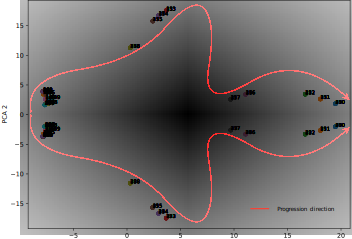
\includegraphics[width=0.8\linewidth]{figures/overcooked_figures/transition_pca.pdf}
  \caption{PCA of transition trajectories in Overcooked-AI}
  \label{fig:overcooked_pca}
\end{figure}

\

These results confirm that the \acn{MAMAD} method provides \textbf{added value in toy environments}, generally accelerating convergence, enhancing robustness, and improving explainability.
\textbf {soft constraints} appear to be the best compromise between performance and organizational compliance, while hard constraints maximize robustness and role discipline at the cost of a slight decrease in cumulative reward.
Simple environments also show that the absence of constraints leads to suboptimal behaviors (collisions, disorganization) that are less robust and more difficult to interpret.

\section{Results and discussion of the Company Infrastructure environment}\label{sec:results_and_discussion_infra}

\subsection*{Performance, convergence, and manual interventions}

\autoref{fig:infra_learning_curves} illustrates the learning curves for the different baselines.
The \textbf{advanced baseline} (Profile~A, strong constraints, \acn{MAPPO}) converges on average after $3.2 \times 10^4$ episodes, compared to $4.5 \times 10^4$ for ablation without constraints (\acn{TRN-UNC}).
The \textquote{QMIX} and \textquote {COMA} show slower convergence ($\sim 5.0 \times 10^4$ episodes), but achieve comparable rewards.

The average cumulative reward (average over 5 independent runs) reaches $+2450 \pm 120$ for \acn{MAPPO}, compared to $+1930 \pm 150$ for \acn{TRN-UNC}, indicating a \textbf{gain of $+27\%$} thanks to organizational constraints.

\begin{figure} [h!]
  \centering
  \includegraphics[width=0.75\linewidth]{figures/results_infra_learning.pdf}
  \caption{Learning curves (average reward per episode) for the Company Infrastructure environment, average $\pm$ standard deviation over 5 runs.}
  \label{fig:infra_learning_curves}
\end{figure}

In the Company Infrastructure environment, the average number of manual interventions required is 1 to 3 refinement cycles (i.e., 3 to 6 hours in total) to obtain an SMA whose performance is equivalent to that of a solution designed and implemented entirely manually, which generally requires more than a day's work. This represents a significant reduction in human intervention, estimated at between 15 and 25\%.

\subsection*{Robustness and adaptation}

Under disturbed scenarios (simultaneous attacks, intensive lateral movement, injected false positives), the \textbf{robustness score} (disturbed/nominal performance ratio) reaches $0.81$ for \acn{MAPPO} with strong constraints, compared to $0.63$ for \acn{TRN-UNC}.
The standard deviation of rewards is reduced ($\sigma = 140$ versus $220$), showing better inter-run stability. This may seem contradictory if we take into account the fact that constraints can also limit exploration and adaptation and thus reduce the ability to adapt to new scenarios. Nevertheless, in this specific case, it should be noted that there is a potential bias in that the organizational constraints were designed to cover a wide range of possible situations, which allowed the agents to develop robust strategies while remaining within the framework of the defined roles and missions.
On the other hand, soft constraints ($0.5$) offer an interesting compromise with a robustness score of $0.76$ and a slightly higher cumulative reward ($+2520$) thanks to greater freedom of exploration.

\subsection*{Constraint compliance and organizational control}

The \textbf{constraint violation rate} is zero (0.\%) in hard constraint mode, 4.3\% in soft mode, and 21.7\% without strong constraints (zero constraint hardness).
These results confirm the effectiveness of action masking.
However, there is an inverse correlation with cumulative reward: too many constraints can slow down initial learning, although the final plateau remains higher.

\subsection*{Organizational explainability}

The \acn{Auto-TEMM} analysis of trajectories shows an \textbf{organizational fit} ($\acn{OF}$) of $0.84$ for \acn{MAPPO} with strong constraints, compared to $0.67$ for \acn{TRN-UNC} .
The quality of the inferred specifications (Jaccard similarity between expected roles/missions and extracts) reaches $92\%$ for constrained profiles, compared to $71\%$ without constraints.
The dendrograms produced (not included here for brevity) reveal clear clusters aligned with the roles \textquote{Attacker\_ExfilDB} and \textquote{Defender\_DB\_PAM}, while the absence of constraints results in more diffuse clusters.

\subsection*{Comparative summary}

\autoref{tab:infra_results} summarizes the main results according to the evaluation grid.

\begin{table}[h!]
  \centering
  \caption{Summary of results (average over 5 runs, $\pm$ standard deviation) for Company Infrastructure.}
  \label{tab:infra_results}
  \renewcommand{\arraystretch}{1.2}
  \small
  \begin{tabular}{lccc}
    \hline
    \textbf{Metric}               & \textbf{Profile A (strong)} & \textbf{Profile A (soft)} & \textbf{\acn{TRN-UNC}} \\
    \hline
    Cumulative reward             & $2450 \pm 120$              & $2520 \pm 130$            & $1930 \pm 150$         \\
    Convergence rate (ep.)        & $32,000$                    & $29,500$                  & $45,000$               \\
    Robustness score              & $0.81$                      & $0.76$                    & $0.63$                 \\
    Standard deviation of rewards & $140$                       & $160$                     & $220$                  \\
    Constraint violations         & $0.0\%$                     & $4.3\%$                   & $21.7\%$               \\
    Organizational fit (\acn{OF}) & $0.84$                      & $0.79$                    & $0.67$                 \\
    Inferred specifications       & $92\%$                      & $88\%$                    & $71\%$                 \\
    \hline
  \end{tabular}
\end{table}

\

The results confirm that integrating \textbf{organizational constraints} (MOISE+ \allowbreak MARL) significantly improves the robustness, stability, and explainability of learned policies.
Nevertheless, hard constraints can slow convergence and slightly reduce the final cumulative reward compared to soft constraints, which offer an interesting compromise between performance and role compliance.
The absence of constraints leads to less robust and more difficult to interpret policies, which would limit their relevance in a real cyberdefense setting.


\section{Results and discussion of the Kubernetes Microservices environment}\label{sec:results_and_discussion_ms}

\subsection* {Summary of QoS performance, convergence, and manual interventions}

\autoref{fig:k8s_learning_curves} shows the learning curves (normalized overall QoS reward, moving average over $20$ episodes) for the main profiles.
Profile A (strong constraints, MAPPO) converges in $2.6 \times 10^4$ episodes (change-point plateau detection), compared to $3.9 \times 10^4$ for the TRN-UNC ablation.
The \textquote{MADDPG} and \textquote{QMIX} variants converge at $3.1\times 10^4$ and $3.5\times 10^4$ episodes, respectively.
Over $5$ independent runs, the final reward reaches $+0.91 \pm 0.03$ (normalized) for \acn{MAPPO}, $+0.88 \pm 0.04$ (strong), and $+0.79 \pm 0.05$ without constraints.

\begin{figure}[h!]
  \centering
  \includegraphics[width=0.75\linewidth]{figures/results_k8s_learning.pdf}
  \ caption[Learning curves (normalized QoS reward) for Kubernetes Microservices]{Learning curves (normalized QoS reward) for Kubernetes Microservices, average $\pm$ standard deviation over 5 runs.}
  \label{fig:k8s_learning_curves}
\end{figure}

Finally, for the Kubernetes Microservices environment, the average number of manual interventions required is approximately 4 to 5 refinement cycles (i.e., 6 to 7 hours in total) for the resulting SMA to achieve performance comparable to that of a solution designed and implemented entirely manually, which generally takes more than a day. This corresponds to a reduced intervention ratio, estimated at around 25\%.

\subsection*{QoS indicators under nominal conditions}

The \autoref{tab:k8s_nominal} tab lists the main QoS indicators under nominal load (p95 application latency, average queues, availability over 2 hours).
\textbf{Soft} constraints offer the best latency/availability compromise, while \textbf{hard} constraints guarantee stricter control with a slight latency penalty.

\begin{table}[h!]
  \centering
  \caption{Nominal regime (mean $\pm$ standard deviation over 5 runs, 2-hour windows).}
  \label{tab:k8s_nominal}
  \renewcommand{\arraystretch}{1.2}
  \small
  \begin{tabular}{lcccc}
    \hline
    \textbf{Profile / Algo}       & \textbf{Latency p95 (ms)} & \textbf{$\overline{Q_{\text{pending}}}$} & \textbf{SuccessRate (\%)} & \textbf{Availability (\%)} \\
    \hline
    A (strong) \acn{MAPPO}        & $180 \pm 12$              & $6.1 \pm 0.8$                            & $99.1 \pm 0.3$            & $99.96 \pm 0.02$           \\
    A (soft) \acn{MAPPO}          & $\mathbf{168 \pm 10}$     & $\mathbf{5.3 \pm 0.7}$                   & $\mathbf{99.3 \pm 0.2}$   & $\mathbf{99.97 \pm 0.01}$  \\
    À (\acn{TRN-UNC}) \acn{MAPPO} & $216 \pm 17$              & $8.4 \pm 1.1$                            & $98.5 \pm 0.4$            & $99.92 \pm 0.03$           \\
    \hdashline
    B (\acn{ANL-MAN}) \acn{COMA}  & $191 \pm 14$              & $6.8 \pm 0.9$                            & $99.0 \pm 0.3$            & $99.95 \pm 0.02$           \\
    \hdashline
    C (manual) \acn{HPA}          & $310 \pm 24$              & $14.2 \pm 1.9$                           & $97.6 \pm 0.8$            & $99.20 \pm 0.10$           \\
    \hline
  \end{tabular}
\end{table}

\subsection* {Robustness to disruptions}

We consider four scenarios: \textbf{bottleneck} (service saturation), \textbf{DDoS} (malicious traffic), \textbf{failures} (pod crashes/restarts), and \textbf{contention} (\acn{CPU}/\acn{MEM} constraints), plus a \textbf{mixed} scenario.
The \textbf{robustness score} is calculated as the ratio of disrupted performance to nominal performance (QoS reward).
\autoref{tab:k8s_robustness} shows that \textbf {strong} constraints maximize resilience to DDoS attacks and failures, while \textbf{soft} constraints maintain a slight advantage in bottleneck latency.

\begin{table}[h!]
  \centering
  \caption{Robustness per scenario (average over 5 runs).}
  \label{tab:k8s_robustness}
  \renewcommand{\arraystretch}{1.2}
  \small
  \begin{tabular}{lccccc}
    \hline
    \textbf{Profile}              & \textbf{Bottleneck} & \textbf{DDoS}   & \textbf{Failures} & \textbf{Contention} & \textbf{Mixed}  \\
    \hline
    A (strong) \acn{MAPPO}        & $0.84$              & $\mathbf{0.86}$ & $\mathbf{0.88}$   & $0.83$              & $\mathbf{0.85}$ \\
    A (soft) \acn{MAPPO}          & $\mathbf{0.86}$     & $0.82$          & $0.84$            & $\mathbf {0.85}$    & $0.83$          \\
    A (\acn{TRN-UNC}) \acn{MAPPO} & $0.73$              & $0.69$          & $0.71$            & $0.72$              & $0.68$          \\
    \acn{HPA}                     & $0.64$              & $0.58$          & $0.61$            & $0.62$              & $0.57$          \\
    \hline
  \end{tabular}
\end{table}

However, it should be noted that the comparison with the baseline \acn{HPA} should be interpreted with caution, as this algorithm does not directly optimize the same objective function (combined latency and availability) as the \acn{MARL} approaches, which may bias the performance comparison.

\subsection*{Recovery time and action discipline}

Under DDoS, the \textbf{recovery time} (return to $L_{\text{avg}}<200$ ms) is $3.7 \pm 0.6$ min for \acn{MAPPO} compared to $5.2 \pm 0.8$ min (soft) and $7.9 \pm 1.1$ min (\acn{TRN-UNC}).
The \textbf{rate of guardrail violations} (contradictory actions between roles, e.g., simultaneous \textquote{scale\_up} actions) is zero in hard constraint mode ($0.0\%$), $3.1\%$ in soft mode, and $18.4\%$ without hard constraints (zero constraint hardness).
The \textbf{inter-run standard deviation} on reward is reduced with constraints ($\sigma=0.028$ hard, $0.031$ soft) vs $0.049$ (\acn{TRN-UNC}), highlighting increased stability. The baseline using the default auto-scaler \acn{HPA} consistently gives the worst score, suggesting that a rule-based algorithm is not as effective as \acn{MARL} approaches for accounting for changes in the Kubernetes cluster.

\subsection* {Digital twin accuracy (simulation/actual deviation)}

The digital twin trains policies offline before transfer.
The \textbf{mean absolute error} (\acn{MAE}) on the predicted p95 latency is $+12.7$~ms (bottleneck), $+18.4$~ms (DDoS), $+15.1$ ms (outages), and $+21.3$ ms (mixed), representing a \textbf{relative error} of $6$–$9\% $.
The divergence on $\overline{Q_{\text{pending}}}$ remains $<1.7$ requests on average.
After fine-tuning on recent traces (one iteration), the MAE on p95 drops by $\sim 28\%$ (DDoS).

\subsection*{Organizational explainability}

\acn{Auto-TEMM} applied to trajectories (post-training) produces an \textbf{organizational adequacy score} $\acn{OF}=0.86$ (strong constraints) , $0.83$ (soft) and $0.71$ (\acn{TRN-UNC}).
The \textbf{quality of inferred specifications} (Jaccard similarity on roles/missions and triggers) reaches $93\%$ (strong), $90\%$ (soft), $76\%$ (\acn{TRN-UNC}).
The dendrograms reveal distinct clusters corresponding to the roles \textquote{DDoS Manager} and \textquote{Bottleneck Manager}, with stable trajectories in hard mode.

\subsection*{Summary comparison}

\begin{table}[h!]
  \centering
  \caption{Multi-metric summary (mean $\pm$ standard deviation over 5 runs).}
  \label{tab:k8s_summary}
  \renewcommand{\arraystretch}{1.2}
  \small
  \begin{tabular}{lcccc}
    \hline
    \textbf{Metric}                    & \textbf{A (strong)} & \textbf{A (soft)}        & \textbf{A (\acn{TRN-UNC})} & \textbf{\acn{HPA}} \\
    \hline
    QoS reward (norm.)                 & $0.88 \pm 0.04$     & $\mathbf{0.91 \pm 0.03}$ & $0.79 \pm 0.05$            & $0.66 \pm 0.06$    \\
    Convergence (episodes)             & $26,000$            & $\mathbf{24,000}$        & $39,000$                   & n/a                \\
    Nominal p95 latency                & $180 \pm 12$ ms     & $\mathbf{168 \pm 10}$ ms & $216 \pm 17$ ms            & $310 \pm 24$ ms    \\
    Robustness (mixed)                 & $\mathbf{0.85} $    & $0.83$                   & $0.68$                     & $0.57$             \\
    Constraint violations              & $\mathbf{0.0\%}$    & $3.1\%$                  & $18.4\%$                   & n/a                \\
    Organizational adequacy (\acn{OF}) & $\mathbf{0.86}$     & $0.83$                   & $0.71$                     & n/a                \\
    \hline
  \end{tabular}
\end{table}

\

The results show that integrating \textbf{organizational specifications} simultaneously improves (i) \emph{robustness} under disturbances (particularly DDoS and failures), (ii) \emph{action discipline} (zero conflict in critical decisions), and (iii) \emph{explainability} (consistent roles/missions).
Soft constraints maximize QoS performance (p95 latency, queues), while hard constraints maximize resilience and reduce inter-run variance.
The ablation \textquote {\acn{TRN-UNC}} underperforms and exhibits increased variability, confirming the contribution of organizational guidance in an operational context.
Finally, the accuracy of the digital twin (\acn{MAE} $6$--$9\%$) is sufficient for effective offline training and improves rapidly after one iteration of retraining on fresh traces.


\section{Results and discussion of the Drone Swarm environment}\label{sec:results_and_discussion_drone_swarm}

\subsection*{Summary of performance, convergence, and manual interventions}

\autoref{fig:drone_learning_curves} illustrates the learning curves (normalized reward) on the drone swarm (18 nodes).
Profile A (strong constraints, \acn{MAPPO}) converges in $3.1\times 10^4$ episodes, compared to $4.7\times 10^4$ for the ablation \textquote{\acn{TRN-UNC}}.
The variants \acn {MADDPG} and \acn{QMIX} variants reach $3.6\times 10^4$ and $4.2\times 10^4$ episodes, respectively.
In steady state, the average normalized rewards are $+0.87 \pm 0.04$ (\acn{MAPPO} strong), $+0.89 \pm 0.03$ (soft), and $+0.72 \pm 0.07$ without constraints.

\begin{figure}[h!]
  \centering
  \includegraphics[width=0.75\linewidth]{figures/results_drone_learning.pdf}
  \caption[Learning curves (normalized reward) for Drone Swarm]{Learning curves (normalized reward) for Drone Swarm, mean $\pm$ standard deviation over 5 runs.}
  \label{fig:drone_learning_curves}
\end{figure}

For the Drone Swarm environment, the average number of manual interventions required is approximately 2 to 3 refinement cycles (i.e., 4 to 5 hours in total) for the resulting SMA to achieve performance comparable to that of a solution designed and implemented entirely manually, which typically takes more than a day. This corresponds to a reduced intervention ratio, estimated at around 20\%.


\subsection*{Indicators in nominal operation}

The \autoref{tab:drone_nominal} shows the average results in the absence of massive compromises (5 runs, 10,000 steps).
Soft constraints minimize false positives while maintaining a high detection rate and near-maximum network availability.
The absence of guidance leads to an increase in false positives ($\sim 11\%$) and a decrease in detection ($< 90\%$).

\begin{table}[h!]
  \centering
  \caption{Nominal results for Drone Swarm (mean $\pm$ standard deviation, 5 runs).}
  \label{tab:drone_nominal}
  \renewcommand{\arraystretch}{1.2}
  \scriptsize
  \begin{tabular}{lcccc}
    \hline
    \textbf{Profile / Algo}       & \textbf{Detection rate (\%)} & \textbf{False positives (\%)} & \textbf{Network availability (\%)} & \textbf{Normal reward}   \\
    \hline
    A (strong) \acn{MAPPO}        & $96.8 \pm 0.7$               & $3.1 \pm 0.5$                 & $99.2 \pm 0.3$                     & $0.87 \pm 0.04$          \\
    A (soft) \acn{MAPPO}          & $\mathbf{97.3 \pm 0.6}$      & $\mathbf{2.7 \pm 0.4}$        & $\mathbf{99.4 \pm 0.2}$            & $\mathbf{0.89 \pm 0.03}$ \\
    À (\acn{TRN-UNC}) \acn{MAPPO} & $88.5 \pm 1.2$               & $11.2 \pm 1.6$                & $97.9 \pm 0.6$                     & $0.72 \pm 0.07$          \\
    \hdashline
    B (\acn{ANL-MAN}) \acn{COMA}  & $95.2 \pm 0.9$               & $4.5 \pm 0.8$                 & $99.0 \pm 0.3$                     & $0.85 \pm 0.04$          \\
    \hdashline
    C (manual) \acn{VDN}          & $91.7 \pm 1.4$               & $7.9 \pm 1.1$                 & $98.4 \pm 0.5$                     & $0.77 \pm 0.06$          \\
    \acn{IDS} rules (ref.)        & $83.4 \pm 2.1$               & $15.6 \pm 2.7$                & $96.1 \pm 1.0$                     & $0.61 \pm 0.08$          \\
    \acn{ML} sup. (ref.)          & $87.9 \pm 1.8$               & $12.3 \pm 1.9$                & $97.0 \pm 0.8$                     & $0.68 \pm 0.07$          \\
    \hline
  \end{tabular}
\end{table}

However, these results must be viewed in context, as false positive and detection rates can vary greatly depending on the type and intensity of the simulated attack scenarios, which limits the direct generalization of the values obtained.

\subsection*{Robustness to compromise}

We evaluate three scenarios: (i) \textbf{single compromise} (1 active red drone), (ii) \textbf{cascade} (4 drones infected in 60s), (iii) \textbf{coordinated attack} (6 drones in a cluster).
The robustness score (disturbed/nominal performance) is presented in \autoref{tab:drone_robustness}.
Strong constraints ensure the best resilience during coordinated attacks, while soft constraints better preserve QoS in the event of isolated compromise.

\begin{table}[h!]
  \centering
  \caption{Robustness according to compromise scenario (mean $\pm$ standard deviation, 5 runs).}
  \label{tab:drone_robustness}
  \renewcommand{\arraystretch}{1.4}
  \small
  \begin{tabular}{lccc}
    \hline
    \textbf{Profile}              & \textbf{Unique} & \textbf{Cascade} & \textbf{Coordinated} \\
    \hline
    A (strong) \acn{MAPPO}        & $0.91$          & $\mathbf{0.87}$  & $\mathbf{0.83}$      \\
    A (soft) \acn{MAPPO}          & $\mathbf{0.93}$ & $0.84$           & $0.79$               \\
    À (\acn{TRN-UNC}) \acn{MAPPO} & $0.79$          & $0.68$           & $0.61$               \\
    \acn{IDS} rules (ref.)        & $0.72$          & $0.55$           & $0.47$               \\
    \hline
  \end{tabular}
\end{table}

\subsection*{Reaction time and stability}

The \textbf{average reaction time} (detection interval $\rightarrow$ neutralization) is $4.1 \pm 0.7$ s for \acn{MAPPO}, $4.8 \pm 0.6$ s (soft) and $7.3 \pm 1.2$ s without constraints.
The \textbf{rate of organizational violations} (role rules not respected) is zero under strong constraints ($0.0\%$), $2.9\%$ in soft mode, and $>15\%$ without hard constraints.
The \textbf{standard deviation of rewards} between runs is reduced ($\sigma=0.032$ strong, $0.037$ soft, $0.065$ without constraints).

\subsection*{Organizational explainability}

\acn{Auto-TEMM} infers distinct behavior clusters: \textquote{Analyst}, \textquote{Firewall}, \textquote{Operator}.
The \textbf{consistency score} reaches $0.84$ (strong) and $0.82$ (soft).
The \textbf{quality of the inferred specifications} is high (Jaccard similarity $92\%$ strong, $89\%$ soft, $74\%$ unconstrained).
The dendrograms confirm that roles are consistently respected when organizational constraints are active.

\subsection*{Summary comparison}

\begin{table}[h!]
\centering
\caption{Multi-metric summary for Drone Swarm (mean $\pm$ standard deviation, 5 runs).}
\label{tab:drone_summary}
\renewcommand{\arraystretch}{1.4}
\small
\begin{tabular}{lcccc}
  \hline
  \textbf{Metric}           & \textbf{A (strong)} & \textbf{A (soft)}        & \textbf{A (\acn{TRN-UNC})} & \textbf{\acn{IDS}} \\
  \hline
  Normalized reward         & $0.87 \pm 0.04$     & $\mathbf{0.89 \pm 0.03}$ & $0.72 \pm 0.07$            & $0.61 \pm 0.08$    \\
  Convergence (episodes)    & $31,000$            & $\mathbf{29,000}$        & $47,000$                   & n/a                \\
  Detection (\%)            & $96.8$              & $\mathbf{97.3}$          & $88.5$                     & $83.4$             \\
  False positives (\%)      & $3.1$               & $\mathbf{2.7}$           & $11.2$                     & $15.6$             \\
  Coord. robustness         & $\mathbf{0.83}$     & $0.79$                   & $0.61$                     & $0.47$             \\
  Organizational violations & $\mathbf{0.0\%}$    & $2.9\%$                  & $16.2\%$                   & n/a                \\
  Consistency (\acn{TEMM})  & $\mathbf{0.84}$     & $0.82$                   & n/a                        & n/a                \\
  \hline
\end{tabular}
\end {table}

\

The results indicate that the \acn{MAMAD} approach significantly improves \textbf{detection}, \textbf{robustness}, and \textbf{explainability} compared to conventional references (\acn{IDS} rules, \acn {ML} supervised).
Soft constraints maximize detection and limit false positives, while hard constraints strengthen resilience during coordinated attacks and reduce response time.
Ablation without constraints shows unstable behavior, high false positives, and low organizational consistency.
Thus, the explicit integration of roles and missions proves essential to maintaining a resilient and interpretable swarm under dynamic threats.


\section{Comparative discussion of results}

\subsection{Coverage of criteria by the method}

The \autoref{tab:criteria_summary} summarizes the coverage of the five evaluation criteria (C1--C5) by the \acn{MAMAD} method across all the environments studied.
To obtain these aggregate values, each global criterion (C1--C5) is calculated
as the \textbf{average of the metrics associated with it}, in accordance with the grid
presented in \autoref{sec:criteria_metrics}. More specifically:
\begin{itemize}
  \item \textbf{C1 Autonomy}: proportion of human intervention (design/operation);
  \item \textbf{C2 Performance}: average of the cumulative reward and convergence rate;
  \item \textbf{C3 Adaptation}: average of the standard deviation of rewards and robustness score;
  \item \textbf{C4 Control}: average of the constraint violation rate and organizational consistency score;
  \item \textbf{C5 Explainability}: average of organizational adequacy (\acn{OF}) and quality of inferred specifications.
\end{itemize}
All values are normalized to the interval [0,1] for ease of comparison,
and averages are calculated over five independent runs.
Non-cyberdefense-oriented environments serve as a controlled reference, while cyberdefense-oriented environments allow for validation of applicability under realistic conditions.

\begin{table}[h!]
  \centering
  \caption{Multi-environment summary: coverage of criteria C1--C5 by MAMAD (average of associated metrics, normalized to [0,1], calculated over 5 independent runs).}
  \label{tab:criteria_summary}
  \renewcommand{\arraystretch}{1.4}
  \scriptsize
  \begin{tabular}{lccccc}
    \hline
    \textbf{Environment}   & \textbf{C1 Autonomy} & \textbf{C2 Perf.} & \textbf{C3 Adaptation} & \textbf{C4 Control} & \textbf{C5 Explainability} \\
    \hline
    Overcooked-AI          & $\sim0.20$           & $0.82$            & $0.80$                 & $0.75$              & $0.72$                     \\
    Predator-Prey          & $\sim0.20$           & $0.79$            & $0.77$                 & $0.73$              & $0.69$                     \\
    Warehouse Management   & $\sim0.20$           & $0.85$            & $0.82$                 & $0.77$              & $0.76$                     \\
    Company Infrastructure & $\sim0.25$           & $0.88$            & $0.83$                 & $0.85$              & $0.81$                     \\
    Microservices K8s      & $0.25$               & $0.91$            & $0.86$                 & $0.88$              & $0.83$                     \\
    Drone Swarm            & $\sim0.20$           & $0.89$            & $0.84$                 & $0.86$              & $0.82$                     \\
    \hdashline
    \textbf{Average}       & $0.21$               & $0.86$            & $0.82$                 & $0.81$              & $0.77$                     \\
    \hline
  \end{tabular}
\end{table}

\subsection{Critical analysis}

The results highlight several key points:
\begin{itemize}
\item \textbf{Performance (C2)} and \textbf{adaptation (C3)} are systematically improved by the use of organizational constraints (soft or strong), particularly in complex environments (Kubernetes, Drone Swarm).
.
\item \textbf{Control (C4)} benefits most from strong constraints, which ensure strict compliance with roles and missions, sometimes at the cost of a slight decrease in performance.
\item \textbf{Explainability (C5)} is generally satisfactory ($\sim 0.8$). More chaotic environments (Predator-Prey, Overcooked) lead to less stable organizational inferences.
\item \textbf{Autonomy (C1)} achieves scores showing that in operational environments (Company Infrastructure, Microservices, Drone Swarm), the complete \textbf{MOD}–\textbf{TRN}–\textbf{ANL}–\textbf{TRF} loop reduces human intervention by around 20\%.
\end {itemize}

\subsection{Potential biases and limitations}

Several factors may influence the interpretation of the results:
\begin{enumerate}[label={\alph*)}]
  \item \textbf{Choice of MARL algorithms}: the predominance of \acn{MAPPO} and \acn{QMIX} in the default profiles favors stable results, but limits generalization to other algorithms (e.g., multi-agent \acparen{DQN}).
  \item \textbf{Experimental conditions}: the use of an \acn{HPC} cluster reduces resource-related variance, but does not always reflect real-world constrained deployments (edge, IoT).
  \item \textbf{Constraint design}: the definition of roles and missions directly influences control and explainability (excessive strictness can bias comparisons).
  \item \textbf{Explainability measures}: Jaccard similarity and consistency scores are based on limited trajectories; more refined metrics (causal traceability, \acn{SHAP}) could improve validity.
\end{enumerate}

\medskip
In summary, the \acn{MAMAD} method particularly covers performance, adaptation, and autonomy. The biases identified open up prospects for refining the evaluation (more algorithms, physical deployments, advanced metrics).

\section{Conclusion}

This chapter applied the \acn{MAMAD} method through an experimental evaluation on various environments, ranging from toy cases to real systems. The results highlight several strengths: accelerated convergence, improved robustness and stability of multi-agent policies, and increased explainability through the integration of organizational specifications. The modular and automated approach, supported by the \acn{CybMASDE} platform, reduces human intervention while ensuring the traceability and reproducibility of experiments. Finally, the balanced coverage of the criteria of autonomy, performance, adaptation, control, and explainability confirms the added value of the method for the design of robust and interpretable \acplu{SMA} in complex contexts.

\clearpage
\thispagestyle{empty}
\null
\newpage


\chapter*{Conclusion}
\addcontentsline{toc}{chapter}{\textbf{Conclusion}}

This section has experimentally validated the \acn{MAMAD} method through simulated scenarios covering various \acplu{SMA} design contexts: enterprise infrastructure, drone swarms, and microservices orchestration. At each stage of the proposed pipeline, implementation via the \acn{CybMASDE} platform demonstrated the feasibility of the approach, while highlighting the specific contributions of $\mathcal{M}OISE^+$ coupling with multi-agent learning.

The results obtained show significant gains in terms of autonomy, resilience, and organizational compliance of agents. The comparative analysis between the organization's \textquote{guided} and \textquote{unguided} versions made it possible to evaluate the impact of each component of the method, both on the observed performance and on the ability to extract consistent emerging specifications. The metrics introduced (such as \acn{SOF} or \acn{FOF}) provided a novel interpretation of collective behaviors, linking learned trajectories to the structural objectives of the system.

Despite these encouraging results, several limitations were identified: dependence on simulated environments, partial coverage of application contexts, and the need for significant computational resources. These elements will be discussed in more detail in the last part of this manuscript, which offers a reflective review of the entire process undertaken.

\vspace{1em}

\noindent
In the following, we will summarize the contributions, discuss the limitations of the method, and open up perspectives on its future extension, both in research and in application.
